\documentclass[12pt, a4paper, onecolumn, twoside]{report}
% File laporan_setting.tex harus Anda sesuaikan dengan informasi Anda.
%
% Template skripsi / tesis ini berdasarkan aturan yang dikeluarkan UI di tahun 2010.
% Yang mengembangkan template ini dari awal hingga saat ini:
% 1. Fahrurrozi Rahman.
% 2. Adreas Febrian, Lia Sadita, Andre Tampubolon, Erik Dominikus.
% 3. Andrew, Daniel Salim (Mat UI 2010).
% 4. Mia Vania (Mat UI 2011).
% 5. Hengki Tasman
% 6. Barry (Mat UI 2010), Maulana (Mat UI 2011)
% 7. Antonio Kevin (Mat UI 2014)*

%*UPDATE: KEPUTUSAN REKTOR NOMOR 2143/SK/R/UI/2017

%NOTE! Remember to do use [\vspace*{-0.25cm}] for enumerate or other listing, so the spacing will be consistent. 
%TO DO NEXT. Change footer font into Arial.

\usepackage[paper=a4paper,headheight=30pt,left=3cm,top=3cm,right=3cm,bottom=3cm]{geometry}
\usepackage{graphicx}
\usepackage{enumerate}
\usepackage{amsmath,amssymb,amsthm}
\usepackage{mathrsfs}
\usepackage{indentfirst} % Kalimat pertama masuk beberapa cm
\usepackage{natbib} % Untuk merujuk pustaka
\usepackage{tocbibind}
%\usepackage{multirow} % Membuat banyak baris dalam 1 baris di tabel
%\usepackage{colortbl} % Membuat tabel berwarna-warni.
\usepackage{caption}
\usepackage{times}
\usepackage{multirow}
\usepackage{subfig}
\usepackage{makecell}
\usepackage{longtable}
\usepackage{fancyhdr} % Membuat header dan footer pada dokumen.
%\usepackage{pdfpages} % Package untuk memasukan berkas pdf sebagai bagian dari dokumen.

\PassOptionsToPackage{hyphens}{url}
\usepackage{hyperref}
\hypersetup{pdfstartview=FitH,pdfview=FitH}

\usepackage{array}
\usepackage{url}
\urlstyle{same}

\usepackage{setspace}
\linespread{1.3} % Jarak baris 1,5

\usepackage[ConnyRevised]{fncychap} % Membantu dalam mengatur jarak antara tepi kertas dengan posisi header.

%-----------------------------------------------------------------------------%
% Konfigurasi
%-----------------------------------------------------------------------------%
\sloppy

\newif\ifpdf
\ifx\pdfoutput\undefined
   \pdffalse
\else
   \pdfoutput=1
   \pdftrue
\fi

% link page numbers in TOC
\makeatletter
\def\contentsline#1#2#3#4{%
  \ifx\\#4\\%
    \csname l@#1\endcsname{#2}{#3}%
  \else
    \csname l@#1\endcsname{%
      \hyper@linkstart{link}{#4}{#2}\hyper@linkend
    }{%
      % same link destination for the page:
      \hyper@linkstart{link}{#4}{#3}\hyper@linkend
      % link destination is the page itself:
      % \hyperpage{#3}%
    }%
  \fi
}

\renewcommand\section{\@startsection {section}{1}{\z@}%
                                  {-3.5ex \@plus -1ex \@minus -.2ex}%
                                  {2.3ex \@plus.2ex}%
                                  {\normalsize \bfseries}}

\renewcommand\subsection{\@startsection{subsection}{2}{\z@}%
                                     {-3.5ex\@plus -1ex \@minus -.2ex}%
                                     {1.5ex \@plus .2ex}%
                                     {\normalsize\bfseries}}
\makeatother

\setcounter{secnumdepth}{3}

\setcounter{tocdepth}{3}

\newcommand{\f}[1]{\textit{#1}}
\newcommand{\bi}[1]{\textbf{\textit{#1}}}
\newcommand{\bo}[1]{\textbf{#1}}

% Perintah untuk membuat perintah/variabel baru.
\newcommand{\var}[2]{\newcommand{#1}{#2}}

% Perintah untuk membuat perintah/variabel baru. Teks yang ditulis dalam
% perintah ini akan diformat ulang menggunakan huruf kapital.
\newcommand{\Var}[2]{\newcommand{#1}{\uppercase{#2}}}

% Tambahkan kata-kata yang dimasukan kedalam Table of Contents.
\newcommand{\addChapter}[1]{\phantomsection \addcontentsline{toc}{chapter}{#1}}

\renewcommand{\bibname}{\normalsize DAFTAR REFERENSI}
\renewcommand{\contentsname}{\normalsize DAFTAR ISI}
\renewcommand{\listfigurename}{\normalsize DAFTAR GAMBAR}
\renewcommand{\listtablename}{\normalsize DAFTAR TABEL}
\renewcommand{\figurename}{\normalsize Gambar}
\renewcommand{\tablename}{\normalsize Tabel}
\renewcommand{\chaptername}{\normalsize BAB}
\def\proofname{Bukti}

\theoremstyle{definition} % Isi teorema tidak ditulis miring
\newtheorem{theorem}{Teorema}[chapter]
\newtheorem{lemma}[theorem]{Lema} 
\newtheorem{proposition}[theorem]{Proposisi}
\newtheorem{corollary}[theorem]{Akibat}
\newtheorem{definition}{Definisi}[chapter]
\newtheorem{example}{Contoh}[chapter]

\newenvironment{remark}[1][Catatan]{\begin{trivlist}
\item[\hskip \labelsep {\normalsize \bfseries #1}]}{\end{trivlist}}

\usepackage{titlesec}
\titlespacing*{\chapter}{0pt}{-32pt}{20pt}
\titleformat{\chapter}[display]{\center \normalsize \bfseries}{\chaptertitlename \, \thechapter}{0pt}{\normalsize} % Memperbaiki judul tiap bab

% Memuat konfigurasi khusus untuk laporan yang sedang dibuat
%-----------------------------------------------------------------------------
% Informasi Mengenai Dokumen
%-----------------------------------------------------------------------------

% Judul laporan.
% Tulis judul Skripsi/Thesis/Disertasi Anda di sini
\var{\judul}{	Pendekatan STATIS dan Dynamic Biplot untuk Analisis Spasio-Temporal Sosio-Ekonomi (Studi Kasus: Provinsi Banten, DKI Jakarta, dan Jawa Barat 2020--2024)}

% Tulis kembali judul laporan, kali ini akan diubah menjadi huruf kapital secara otomatis
% Tulis judul Skripsi/Thesis/Disertasi Anda di sini
\Var{\Judul}{Pendekatan STATIS dan Dynamic Biplot untuk Analisis Spasio-Temporal Sosio-Ekonomi (Studi Kasus: Provinsi Banten, DKI Jakarta, dan Jawa Barat 2020--2024)}

% Tulis kembali judul laporan namun dengan bahasa Ingris
\var{\judulInggris}{STATIC and Dynamic Biplot Approaches for Socio-Economic Spatio-Temporal Analysis (Case Studies: Province of Banten, DKI Jakarta, and West Java 2020--2024)}

% Tipe laporan, dapat berisi Skripsi, Tesis atau Disertasi
\var{\type}{Skripsi} % Pilih satu, hapus yang tidak perlu
\Var{\Type}{Skripsi} % Pilih satu, hapus yang tidak perlu, Akan jadi huruf besar semua secara otomatis

% Tulis nama penulis
\var{\penulis}{Ammar Hanafi}
\Var{\Penulis}{Ammar Hanafi} % Akan jadi huruf besar semua secara otomatis

% Tulis NPM penulis
\var{\npm}{2206051582}

% Tuliskan Fakultas dimana penulis berada
\Var{\Fakultas}{Matematika dan Ilmu Pengetahuan Alam}
\var{\fakultas}{Matematika dan Ilmu Pengetahuan Alam}

% Tuliskan Program Studi yang diambil penulis
\Var{\Program}{Sarjana Statistika}
\var{\program}{Sarjana Statistika}

% Tuliskan Program Studi yang diambil penulis, dalam bahasa Inggris
\Var{\Programinggris}{Undergraduate Study Program of Statistics}
\var{\programinggris}{Undergraduate Study Program of Statistics}

% Tuliskan bulan dan tahun publikasi laporan
\Var{\bulanTahun}{Juni 2026}
\var{\tahun}{2026}

% Tuliskan gelar yang akan diperoleh dengan menyerahkan laporan ini
\var{\gelar}{Sarjana} % Pilih satu, hapus yang tidak perlu

% Tuliskan tanggal pengesahan laporan, waktu dimana laporan diserahkan ke
% penguji/sekretariat
\var{\tanggalPengesahan}{17 Juli 2026}

% Tuliskan tanggal keputusan sidang dikeluarkan dan penulis dinyatakan lulus/tidak lulus
\var{\tanggalLulus}{17 Juli 2026}

% Tuliskan nama pembimbing
\var{\pembimbinga}{Dr. Dra. Yekti Widyaningsih, M.Si.}
% \var{\pembimbingb}{Nama Pembimbing II} % Beri tanda % di awal baris ini jika Anda tidak punya Pembimbing II skripsi

%Tuliskan nama penguji
\var{\pengujia}{Sarini Abdullah, S.Si., M.Stats., Ph.D.}
\var{\pengujib}{Gianinna Ardaneswari, S.Si., M.Si.}
 % Anda HARUS edit file laporan_setting.tex

% Memuat Daftar pemenggalan suku kata dan istilah dalam LaTeX
%
% Hyphenation untuk Indonesia
%
% @author  Andreas Febrian
% @version 1.00
%
% Tambahkan cara pemenggalan kata-kata yang salah dipenggal secara otomatis
% oleh LaTeX. Jika kata tersebut dapat dipenggal dengan benar, maka tidak
% perlu ditambahkan dalam berkas ini. Tanda pemenggalan kata menggunakan
% tanda '-'; contoh:
% menarik
%   --> pemenggalan: me-na-rik
%

\hyphenation{
    % alphabhet A
    aki-bat
    ana-li-sis
    ana-li-tik
    ang-go-ta
    an-ti-bio-tik
    % alphabhet B
    ba-gai-ma-na
    be-be-ra-pa
    ber-ge-rak
    ber-hu-bu-ngan
    ber-pe-nga-ruh
    ber-te-ri-ma
    bi-la-ngan
    bim-bi-ngan
    % alphabhet C
    % alphabhet D
    de-fi-ni-si
    de-ngan
    di-ban-ding-kan
    dia-gram
    di-ba-ngun
    di-buk-ti-kan
    di-da-pat-kan
    di-de-fi-ni-si-kan
    di-fe-ren-si-al
    di-ha-rap-kan
    di-li-hat
    di-mo-del-kan
    di-mu-lai
    di-nya-ta-kan
    di-pe-nga-ru-hi
    di-sa-ji-kan
    di-re-pre-sen-ta-si-kan
    di-ting-kat-kan
    du-ku-ngan
    % alphabhet E
    eks-pli-sit
    eks-pre-si
    eva-lua-si
    % alphabhet F
    frak-sio-nal
    % alphabhet G
    geo-me-tri
    % alphabhet H
    ha-rap
    hi-tung
    % alphabhet I
    im-pli-sit
    in-te-gral
    ite-ra-si
    ite-ra-tif
    % alphabhet J
    % alphabhet K
    ka-it
    ke-mung-kin-an
    ke-se-im-ba-ngan
    ke-se-tim-ba-ngan
    ki-rim
    kom-par-te-men
    kon-fi-gu-ra-si
    kon-struk-si
    % alphabhet L
    li-mit
    li-te-ra-tur
    % alphabhet M
    ma-te-ma-ti-ka
    me-mo-del-kan
    me-mo-ri
    men-de-ngar-kan
    me-ne-ri-ma
    me-nga-it-kan
    me-nga-ju-kan
    me-nga-la-mi
    me-nga-na-li-sis
    me-nga-pa
    me-nga-rah-kan
    meng-ar-ti-kan
    me-nge-nai
    me-ngi-rim-kan
    me-nya-ta-kan
    mi-sal
    mi-sal-kan
    mo-del
    mu-lai
    mung-kin
    % alphabhet N
    na-pas
    non-eks-klu-sif
    % alphabhet O
    ope-ra-tor
    % alphabhet P
    pa-ling
    pa-ra-me-ter
    pa-sang
    pa-sang-an
    pe-mo-del-an
    pe-nga-ruh
    pe-nga-wa-san
    pe-ngem-ba-ngan
    pe-ngo-bat-an
    pen-ting
    pe-ngu-ra-ngan
    pe-nye-le-sai-an
    per-ge-rak-an
    per-hi-tung-an
    pe-ri-la-ku
    per-ten-ta-ngan
    per-u-mum-an
    peru-ba-han
    po-pu-la-si
    pro-duk-ti-vi-tas
	% alphabhet Q
    % alphabhet R
    re-pre-sen-ta-si
    % alphabhet S
    sa-ngat
    sa-tu
    sa-tu-nya
    se-dang
    se-dang-kan
    se-ki-tar
    se-ring
    si-mu-la-si
    su-a-tu
    sub-sti-tu-si
    % alphabhet T
    ten-tang
    te-ra-pi
    te-ri-ma
    tri-li-un
    tu-run-an
    % alphabhet U
    % alphabhet V
    % alphabhet W
    % alphabhet X
    % alphabhet Y
    % alphabhet Z
    % special
}  % Tambahkan daftar pemenggalan kata dalam file hype.indonesia.tex

% Memuat Daftar istilah yang mungkin perlu ditandai
%
% @author  Andreas Febrian
% @version 1.00
% 
% Mendaftar seluruh istilah yang mungkin akan perlu dijadikan 
% italic atau bold pada setiap kemunculannya dalam dokumen. 
% 

\var{\license}{\f{Creative Common License 1.0 Generic}}
\var{\bslash}{$\setminus$}

\begin{document}

% Sampul Depan Skripsi / Tesis
%
% Sampul Laporan

%
% @author  unknown
% @version 1.01
% @edit by Andreas Febrian
%

\begin{titlepage}
    \begin{center}    
        \begin{figure}
            \begin{center}
                
\includegraphics[width=2.5cm]{pics/makara.png}
            \end{center}
        \end{figure}    
        \vspace*{0cm}
        \bo{
        	UNIVERSITAS INDONESIA\\
        }
        
        \vspace*{1.0cm}
        % judul thesis harus dalam 14pt Times New Roman
        \bo{\Judul} \\[1.0cm]

        \vspace*{2.5 cm}    
        % harus dalam 14pt Times New Roman
        \bo{\Type}

        \vspace*{3 cm}       
        % penulis dan npm
        \bo{\Penulis} \\
        \bo{\npm} \\

        \vspace*{5.0cm}

        % informasi mengenai fakultas dan program studi
        \bo{
        	FAKULTAS \Fakultas\\
        	PROGRAM STUDI \Jenjang~\Bidang \\
        	Kota Depok \\
        	\bulanTahun
            }
    \end{center}
\end{titlepage}
 % Dilarang mengubah isi file sampul.tex 

\pagenumbering{roman} % Gunakan penomoran halaman romawi

%pengaturan headerfooterhalaman
\renewcommand{\headrulewidth}{0.0pt}
	\fancyhf{}
	\fancyhead[L]{}
	\fancyhead[C]{}
	\fancyhead[R]{}
	\renewcommand{\headrulewidth}{0.0pt}
	\fancyfoot[C]{\thepage}
	\renewcommand{\footrulewidth}{0pt}
\pagestyle{fancy}

% Memuat halaman judul dalam
\addChapter{HALAMAN JUDUL}
%
% Halaman Judul Laporan 
%
% @author  unknown
% @version 1.01
% @edit by Andreas Febrian
%

\begin{titlepage}
    \begin{center}\begin{figure}
            \begin{center}
                
\includegraphics[width=2.5cm]{pics/makara.png}
            \end{center}
        \end{figure}    
        \vspace*{0cm}
        \bo{
        	UNIVERSITAS INDONESIA\\
        }
        
        \vspace*{1.0cm}
        % judul thesis harus dalam 14pt Times New Roman
        \bo{\Judul} \\[1.0cm]

        \vspace*{2.5 cm}    
        % harus dalam 14pt Times New Roman
        \bo{\Type} \\
        % keterangan prasyarat
        \bo{Diajukan sebagai salah satu syarat untuk memperoleh gelar \\
        \gelar}\\

        \vspace*{3 cm}       
        % penulis dan npm
        \bo{\Penulis} \\
        \bo{\npm} \\

        \vspace*{3.5cm}

        % informasi mengenai fakultas dan program studi
        \bo{
        	FAKULTAS \Fakultas\\
        	PROGRAM STUDI \Program \\
        	DEPOK \\
        	\bulanTahun
        }
    \end{center}
\end{titlepage} % Dilarang mengubah isi file judul_dalam.tex

\setcounter{page}{2} % nomor halaman selanjutnya adalah 2

% Memuat halaman pengesahan
%\addChapter{LEMBAR PERSETUJUAN}
%%
% Halaman Pengesahan
%
% @author  Andreas Febrian
% @version 1.01
%

\chapter*{\normalsize HALAMAN PERSETUJUAN}

\vspace*{0.2cm}

\noindent
\begin{tabular}{l l p{11cm}}
	Judul&: & \judul \\
	Nama&: & \penulis \\
	NPM&: & \npm \\
\end{tabular} \\

\vspace*{1.2cm}

\noindent Laporan \type~ini telah diperiksa dan disetujui.\\[0.3cm]
\begin{center}
\tanggalPengesahan \\[2cm]


\underline{\pembimbinga}\\[0.1cm]
Pembimbing \type
\end{center}

\newpage  % Dilarang mengubah isi file pengesahan.tex 

% load halaman orisinalitas
\addChapter{HALAMAN PERNYATAAN ORISINALITAS}
%
% Halaman Orisinalitas
%
% @author  Andreas Febrian
% @version 1.01
%

\chapter*{\normalsize HALAMAN PERNYATAAN ORISINALITAS}
\vspace*{2cm}
\begin{doublespace}
\begin{center}
	\bo{\type~ini adalah hasil karya saya sendiri, \\
	dan semua sumber baik yang dikutip maupun dirujuk \\
	telah saya nyatakan dengan benar.} \\
	\vspace*{2.6cm}
	
	\begin{tabular}{l c l}
	\bo{Nama} & \bo{:} & \bo{\penulis} \\
	\bo{NPM} & \bo{:} & \bo{\npm} \\
	\end{tabular}
	
	\bigskip
	
	\centerline{\bo{Tanda Tangan}}
	
	\vskip 2cm
	
	\begin{tabular}{l c l}
	\bo{Tanggal} & \bo{:} & \bo{\tanggalPengesahan} \\
	\end{tabular}
\end{center}
\end{doublespace}

\newpage  % Dilarang mengubah isi file orisinal.tex

%pengaturan rata kiri
%\raggedright
\setlength\parindent{0.7cm}

\addChapter{HALAMAN PENGESAHAN}
%
% Halaman Pengesahan Sidang
%
% @author  Andreas Febrian, Andre Tampubolon
% @version 1.02
%

\chapter*{\normalsize HALAMAN PENGESAHAN}
\begin{singlespace}
\vspace*{0.4cm}
\noindent

\noindent
\begin{tabular}{ll p{9cm}}
	\type~ini diajukan oleh&: & \\ % ---- Jangan diedit ----
	Nama&: & \penulis \\ % ---- Jangan diedit ----
	NPM&: & \npm \\ % ---- Jangan diedit ----
	Program Studi&: & \program \\ % ---- Jangan diedit ----
	Judul \type&: & \judul \\ % ---- Jangan diedit ----
\end{tabular} \\

\vspace*{1.0cm}

\noindent Telah berhasil dipertahankan di hadapan Dewan Penguji
dan diterima sebagai bagian persyaratan yang diperlukan untuk
memperoleh gelar \gelar \, pada Program Studi \program, Fakultas
\fakultas, Universitas Indonesia.\\[0.2cm] % ---- Jangan diedit ----

\begin{center}
	DEWAN PENGUJI
\end{center}

\vspace*{0.3cm}

\begin{tabular}{l l l l }
& & & \\
Pembimbing I &: & \pembimbinga & (\hspace*{3.0cm}) \\ % ---- Jangan diubah ----

% \vspace{0.7cm}

% & & & \\


% Pembimbing II&: & \pembimbingb & (\hspace*{3.0cm}) \\ % ---- Silakan hapus bagian ini jika tidak ada pembimbing II

\vspace{0.7cm}

& & & \\


Penguji I&: & \pengujia & (\hspace*{3.0cm}) \\ % ---- Jangan diubah ------

\vspace{0.7cm}

& & & \\


Penguji II&: & \pengujib & (\hspace*{3.0cm}) \\ % ---- Jangan diubah ------
& & & \\
\end{tabular}\\

\vspace*{2.0cm}

\begin{tabular}{ll l}
	Ditetapkan di&: & Depok\\ % ---- Jangan diedit ----
	Tanggal&: & \tanggalLulus \\ % ---- Jangan diedit ----
\end{tabular}
\end{singlespace}

\newpage  % File pengesahan_sidang.tex mungkin perlu diubah sesuai dengan banyaknya pembimbing dan penguji kolokium atau sidang Anda

\addChapter{KATA PENGANTAR}
%-----------------------------------------------------------------------------%
\chapter*{\normalsize KATA PENGANTAR}
%-----------------------------------------------------------------------------%

Puji syukur kepada Tuhan Yang Maha Esa atas segala berkat dan rahmat-Nya, sehingga penulis dapat menyelesaikan skripsi ini dengan sebaik-baiknya. Selama masa penulisan skripsi ini, penulis telah mendapat banyak dukungan, doa, bantuan, inspirasi, dan motivasi dari berbagai pihak. Untuk itu, penulis ingin berterima kasih kepada:
\begin{enumerate}
	\item Semua staf pengajar atas ilmu pengetahuan yang telah diberikan kepada penulis selama masa kuliah.
	\item Seluruh staf karyawan yang selalu melakukan tugas mereka dengan baik, sehingga memberikan kenyamanan pelayanan bagi siapa saja.
	\item Seluruh teman-teman angkatan 2022 atas semangat, canda tawa dan banyak hal penting selama masa kuliah.
	\item Kakak-kakak angkatan 2021, 2020, dan 2019 serta adik-adik angkatan 2023, dan 2024 yang terus memberi semangat.
\end{enumerate}

\vspace*{0.1cm}

\begin{flushright}
\penulis \\[0.1cm]
\vspace*{0.2cm}
\tahun
\end{flushright}  % Anda HARUS isi file pengantar.tex -------------

\addChapter{HALAMAN PERSETUJUAN PUBLIKASI ILMIAH}
%
% @author  Andre Tampubolon, Andreas Febrian
% @version 1.01
%

\chapter*{\normalsize HALAMAN PERNYATAAN PERSETUJUAN PUBLIKASI TUGAS AKHIR UNTUK KEPENTINGAN AKADEMIS}

\vspace{-0.6cm}

\noindent \rule{15cm}{3pt}

\begin{singlespace}
\vspace*{0.2cm}
\noindent
Sebagai sivitas akademik Universitas Indonesia, saya yang bertanda tangan di bawah ini:
\vspace*{0.4cm}

\begin{flushleft}

\begin{tabular}{p{3cm} l p{8cm}}
	Nama & : & \penulis \\ 	
	NPM & : & \npm \\
	Program Studi & : & \program\\	
	Fakultas & : & \fakultas\\
	Jenis Karya & : & \type \\
\end{tabular}
\end{flushleft}

\noindent demi pengembangan ilmu pengetahuan, menyetujui untuk memberikan
kepada Universitas Indonesia \bo{Hak Bebas Royalti Noneksklusif
(\textit{Non-exclusive Royalty Free Right})} atas karya ilmiah saya yang berjudul:
\begin{center}
	\judul
\end{center}
beserta perangkat yang ada (jika diperlukan). Dengan Hak Bebas Royalti
Noneksklusif ini, Universitas Indonesia berhak menyimpan,
mengalihmedia/formatkan, mengelola dalam bentuk pangkalan data
(\textit{data base}), merawat, dan memublikasikan tugas akhir saya selama
tetap mencantumkan nama saya sebagai penulis/pencipta dan sebagai
pemilik Hak Cipta. \\

\noindent Demikian pernyataan ini saya buat dengan sebenarnya.

\begin{center}
	\vspace*{0.8cm}
	\begin{tabular}{lll}
		Dibuat di&: & Kota Depok \\
		Pada tanggal&: & \tanggalPengesahan \\
	\end{tabular}\\

	\vspace*{0.2cm}
	Yang menyatakan \\
	\vspace{-0.2cm}
	\includegraphics[width=3cm]{\ttd} \\
	\vspace{-0.2cm}
	(\penulis)
\end{center}
\end{singlespace}

\newpage

 % Dilarang ubah file persetujuan_publikasi.tex 

%pengaturan header footer halaman
\renewcommand{\headrulewidth}{0.0pt}
	\fancyhf{}
	\fancyhead[L]{}
	\fancyhead[C]{}
	\fancyhead[R]{}
	\renewcommand{\headrulewidth}{0.0pt}
	\fancyfoot[C]{\thepage}
	\fancyfoot[R]{{\fontfamily{phv}\selectfont\footnotesize \bo{Universitas Indonesia}}}
	\renewcommand{\footrulewidth}{0.0pt}
\pagestyle{fancyplain}

\addChapter{ABSTRAK}
%
% Halaman Abstrak
%
% @author  Andreas Febrian
% @version 1.00
%

\chapter*{\normalsize ABSTRAK}
\begin{singlespace}
\vspace*{0.2cm}

\noindent\begin{tabular}{l l >{\raggedright\arraybackslash}p{10cm}}
Nama&: & \penulis \\ % Jangan diubah
Program Studi&: & \jenjang~\bidang \\ % Jangan diubah
Judul&: & \judul \\ % Jangan diubah
\end{tabular}

\vspace*{0.5cm}

\noindent

Wilayah strategis Banten, DKI Jakarta, dan Jawa Barat sebagai pusat ekonomi nasional mengalami perubahan struktural kompleks selama 2020--2024 akibat pandemi COVID-19 dan fase pemulihan yang tidak merata antar-kabupaten/kota; pendekatan multivariat konvensional memiliki keterbatasan dalam menangkap interaksi simultan antara dimensi spasial, indikator sosial-ekonomi, dan pergeseran temporal secara terpadu. Penelitian ini bertujuan mengevaluasi stabilitas longitudinal pada periode saat pandemi (2020--2021) dan pasca pandemi (2022--2024), serta memetakan trajektori spasio-temporal sebelas indikator pembangunan strategis yang meliputi aspek ekonomi (PDRB), kesejahteraan (Kemiskinan, Garis Kemiskinan, Pangan), pembangunan manusia (Pendidikan, Kesehatan), ketenagakerjaan, serta kesetaraan (Gender, Gini Ratio) di 41 kabupaten/kota pada ketiga provinsi tersebut. Metode STATIS (\textit{Structuration des Tableaux à Trois Indices de la Statistique} atau Strukturisasi Tabel dengan Tiga Indeks dalam Statistik) diterapkan melalui tahapan: (1)~standardisasi $Z$-\textit{score} terbobot demografis menggunakan jumlah penduduk sebagai bobot metrik, (2)~evaluasi inter-struktur menggunakan koefisien $RV$ untuk mengukur kemiripan antar-tabel tahunan, (3)~pembentukan struktur kompromi ($\mathbf{W}_c$) melalui pembobotan spektral optimal, (4)~validasi signifikansi via uji permutasi Monte Carlo, dan (5)~visualisasi lintasan (\textit{trajectory}) menggunakan \textit{Dynamic Biplot}; pengelompokan lanjutan diterapkan melalui algoritma \textit{K-Means} ($k=3$) pada koordinat kompromi yang direduksi via \textit{Principal Component Analysis} (PCA). Analisis inter-struktur menunjukkan konsistensi yang sangat tinggi dengan seluruh koefisien $RV$ melampaui ambang batas kritis dan terbukti signifikan secara statistik, membuktikan bahwa hierarki relatif antar-wilayah tetap stabil meskipun terjadi fluktuasi absolut akibat pandemi; struktur kompromi mampu menjelaskan sebagian besar total variansi melalui dua dimensi utama, yaitu Dimensi~1 yang merepresentasikan "Kapasitas Sosio-Ekonomi" (berkorelasi kuat dengan PDRB dan IPM) dan Dimensi~2 yang mencerminkan "Tekanan Pasar Tenaga Kerja" (didominasi Tingkat Pengangguran Terbuka). \textit{Dynamic Biplot} mengidentifikasi tiga pola trajektori: pemulihan berbentuk~V pada pusat metropolitan berbasis jasa, trajektori stagnan di kabupaten selatan Banten dan Jawa Barat, serta pertumbuhan progresif di wilayah penyangga; pengelompokan \textit{K-Means} menghasilkan tiga klaster yaitu "Maju," "Berkembang," dan "Tertinggal" yang memiliki keselarasan tinggi dengan kategori normatif IPM UNDP, mengindikasikan bahwa kesenjangan regional bersumber dari faktor struktural yang persisten. Penelitian ini dibatasi pada tiga provinsi di Jawa bagian Barat dengan sebelas indikator terpilih dan rentang waktu lima tahun (2020--2024); kebaruan penelitian ini terletak pada penerapan metode STATIS untuk analisis dinamika pembangunan regional pada periode saat dan pasca pandemi COVID-19 di konteks Jawa bagian Barat, yang diintegrasikan dengan sistem \textit{dashboard} web interaktif berbasis Python mencakup uji diagnostik, visualisasi klaster spasio-temporal, serta ekspor otomatis sebagai instrumen analitik bagi peneliti maupun pemangku kebijakan.

\bigskip

\noindent

\vspace*{0.5cm}

\noindent \bo{Kata kunci}:
	Analisis Data Tiga Arah, Data Longitudinal, \textit{K-Means Clustering}, PCA, Visualisasi Interaktif.
\end{singlespace}
\newpage  % Abstrak dalam bahasa Indonesia. Ubah file abstrak.tex.

\addChapter{ABSTRACT}
%
% Halaman Abstract
%
% @author  Andreas Febrian
% @version 1.00
%

\chapter*{\normalsize ABSTRACT}
\begin{singlespace}
\vspace*{0.2cm}

\noindent \begin{tabular}{l l >{\raggedright\arraybackslash}p{11.0cm}}
	Name&: & \penulis \\ % ------------ Jangan diedit
	Program&: & \jenjanginggris~Study Program of~\bidanginggris \\ % ------------ Jangan diedit
	Title&: & \judulInggris \\ % ------------ Jangan diedit
\end{tabular}

\vspace*{0.5cm}

\noindent

The development dynamics in the strategic regions of Banten, DKI Jakarta, and West Java exhibited high complexity during the 2020--2024 period. As the center of national economic agglomeration, these three provinces experienced simultaneous changes due to the COVID-19 pandemic, followed by an uneven recovery phase across regencies/cities. These changes occurred not only in macroeconomic indicators but also propagated to dimensions of social welfare and human capital quality. To thoroughly understand the evolution of the structural relationships among these indicators, a three-way data analysis approach capable of capturing spatio-temporal interaction patterns is required.

This research applies the STATIS (\textit{Structuration des Tableaux à Trois Indices de la Statistique}) method to analyze the dynamics of 12 strategic development indicators---covering economic aspects (GRDP), welfare (Poverty, Poverty Line, Food), human development (HDI, Education, Health), labor, and equality (Gender, Gini Ratio)---across all regencies/cities in the three provinces. The analysis centers on the formation of a compromise structure. Referring to the definition by \citet{lavit94}, the compromise structure ($\mathbf{W}_c$) is constructed as a weighted sum of annual intra-structure matrices, where the weights ($\alpha_k$) are determined based on spectral decomposition to maximize inter-year similarity. This structure represents the most dominant and stable inter-regional relationship patterns during the observation period. Furthermore, this study tests the significance of the structure's stability using permutation tests and integrates the Dynamic Biplot concept to visualize the movement trajectories of regencies/cities from the crisis to the recovery period in a low-dimensional space.

The entire analysis procedure, from data pre-processing to visualization, is implemented using the Python programming language within an interactive web dashboard. This system provides a comprehensive suite of analysis features, ranging from diagnostic tests (KMO, Bartlett) and STATIS analysis to spatio-temporal cluster evaluation (Elbow Method, Dendrograms, Transition Matrices). Through interactive features such as baseline rotation, regional trajectory filtering, and automatic integration of results into LaTeX. This application serves as a sophisticated analytical and visual tool for researchers and policymakers to monitor resilience and accelerate regional development equity in the post-pandemic era.

\vspace*{0.2cm}

\noindent \bo{Keywords}:
	Interactive Visualization, K-Means Clustering, Panel Data, Regional Development, Spatial Autocorrelation, Three-way Analysis. % ------------ Jangan lupa diedit
\end{singlespace}

\newpage  % Abstrak dalam bahasa Inggris. Ubah file abstract.tex.

% Daftar isi, gambar, dan tabel
\tableofcontents
\clearpage

\listoftables % jika ada tabel
\clearpage

\listoffigures % jika ada gambar
\clearpage{\thispagestyle{empty}\cleardoublepage}

% Gunakan penomoran Arab (1, 2, 3, ...) setelah bagian ini.
\pagenumbering{arabic}
%pengaturan headerfooter halaman
\renewcommand{\headrulewidth}{0.0pt}
   \fancyhf{}
	\fancyhead[RO,LE]{\thepage}
	\renewcommand{\headrulewidth}{0.0pt}
	\fancyfoot[R]{\footnotesize \bo{Universitas Indonesia}}
	\renewcommand{\footrulewidth}{0.0pt}
\pagestyle{fancy}

\fancypagestyle{plain}{ %
  \fancyhf{} 
  	\fancyhead[L]{}
  	\fancyhead[C]{}
  	\fancyhead[R]{}
  	\renewcommand{\headrulewidth}{0pt} 
  	\fancyfoot[C]{\thepage}
  	\fancyfoot[R]{\footnotesize \bo{Universitas Indonesia}}
  	\renewcommand{\footrulewidth}{0pt}
}

\clearpage{\thispagestyle{empty}\cleardoublepage}
\chapter{\normalsize PENDAHULUAN}

%-----------------------------------------------------------------------------%
\section{\normalsize Latar Belakang}
%-----------------------------------------------------------------------------%
Kawasan strategis yang meliputi Provinsi Banten, DKI Jakarta, dan Jawa Barat tidak hanya berperan sebagai mesin pertumbuhan ekonomi nasional, tetapi juga menjadi arena dinamika pembangunan manusia yang sangat kompleks dalam lima tahun terakhir. Meskipun wilayah ini memberikan kontribusi yang sangat dominan terhadap perekonomian nasional dengan rata-rata pangsa Produk Domestik Regional Bruto (PDRB) berkisar 33,8 persen dari PDRB Indonesia \citet{bpspdrb}---keberhasilan pembangunannya tidak dapat lagi diukur hanya melalui kacamata indikator makro ekonomi semata. Terdapat interaksi multidimensi yang melibatkan kualitas hidup yang tecermin dalam Indeks Pembangunan Manusia (IPM), Indeks Pembangunan Gender (IPG), serta tantangan kesejahteraan sosial seperti kemiskinan dan ketahanan pangan yang terus mengalami perubahan. Kompleksitas ini menuntut pembuktian empiris yang lebih mendalam untuk melihat bagaimana indikator-indikator tersebut terdistribusi secara nyata di seluruh kabupaten/kota.

Secara empiris, lanskap pembangunan di ketiga provinsi ini menunjukkan polarisasi yang tajam antara pusat-pusat pertumbuhan utama dan wilayah penyangga. Meskipun data PDRB di kota-kota besar mencatat performa ekonomi yang kuat dengan nilai mencapai 532.606,87 miliar rupiah \citet{bpspdrb}, capaian tersebut tidak serta-merta diikuti oleh pemerataan kesejahteraan. Hal ini terlihat dari variasi spasial yang mencolok (\textit{striking spatial variation}) pada indikator kemiskinan, di mana Persentase Penduduk Miskin (PPM) terentang lebar dari 2,29 persen hingga mencapai 15,06 persen di wilayah lainnya. Kesenjangan ini juga terkonfirmasi oleh indikator daya beli, terlihat dari perbedaan Garis Kemiskinan (GK) dan Prevalensi Ketidakcukupan Konsumsi Pangan (PKKP) yang bervariasi lebar antarwilayah \cite{bpspkkp}. Lebih jauh lagi, disparitas kapabilitas manusia juga terlihat mencolok; Rata-rata Lama Sekolah (RLS) dan Angka Harapan Hidup (AHH) masih menunjukkan perbedaan yang nyata. Indeks Pembangunan Gender (IPG) serta Tingkat Pengangguran Terbuka (TPT) masih berada di kisaran 6,55--10,12 persen pada rentang tahun 2020--2024. Namun, persoalan ketimpangan antarwilayah ini menjadi semakin rumit ketika diletakkan dalam konteks waktu yang penuh perubahan.

Selain disparitas spasial, tantangan analisis meningkat akibat adanya dinamika temporal yang sangat fluktuatif sepanjang periode 2020--2024. Periode ini diawali dengan peristiwa pandemi COVID-19 yang menekan indikator makroekonomi dan kesejahteraan secara serentak terlihat dari perubahan pertumbuhan ekonomi yang sempat mencapai angka 1,88 persen pada tahun 2020 \citet{bpspdrb} namun diikuti oleh pola pemulihan yang lajunya tidak seragam di setiap daerah pada tahun-tahun berikutnya. Perubahan drastis dari masa pandemi COVID-19 menuju masa pemulihan ini diduga kuat telah mengubah struktur hubungan antar-indikator secara fundamental; sebagai contoh, pola korelasi antara pertumbuhan ekonomi (PDRB) dengan tingkat pengangguran (TPT) saat krisis sangat mungkin berbeda dibandingkan saat kondisi normal kembali pulih pada tahun 2023--2024. Oleh karena itu, pendekatan analisis multivariat klasik yang mengasumsikan struktur hubungan variabel bersifat statis (tetap sepanjang waktu) menjadi tidak lagi relevan untuk menganalisis fenomena pada periode yang penuh fluktuasi ini.

Untuk mengatasi keterbatasan asumsi stabilitas tersebut, diperlukan pendekatan analisis data tiga-arah (\textit{three-way data analysis}) yang mampu menangani struktur data kompleks yang terdiri dari objek (kabupaten/kota), variabel (indikator sosio-ekonomi), dan situasi (waktu). Penelitian ini mengusulkan penggunaan metode STATIS (\textit{Structuration des Tableaux à Trois Indices de la Statistique}), sebuah metode eksploratif yang diperkenalkan oleh \citet{lavit94,oliveira2024}. Berbeda dengan Analisis Komponen Utama (PCA) konvensional yang hanya bekerja pada data dua dimensi, STATIS dirancang khusus untuk mengekstraksi informasi dari sekumpulan tabel data yang berubah seiring waktu. Metode ini memiliki keunggulan dalam membentuk sebuah struktur kompromi (\textit{compromise structure}) yang merepresentasikan pola hubungan umum antar-indikator selama periode pengamatan, sekaligus memungkinkan identifikasi seberapa jauh struktur ekonomi setiap tahunnya menyimpang dari pola umum tersebut.

Meskipun metode STATIS mampu menghasilkan struktur kompromi secara matematis, kompleksitas hasil analisis dari matriks berdimensi tinggi sering kali sulit dipahami jika hanya disajikan dalam bentuk tabel numerik. Oleh karena itu, penelitian ini mengintegrasikan pendekatan STATIS dengan teknik visualisasi \textit{Dynamic Biplot}. Pendekatan ini memungkinkan proyeksi posisi objek (kabupaten/kota) dan variabel (indikator ekonomi) ke dalam ruang berdimensi rendah, sekaligus menggambarkan pergerakan atau lintasan (\textit{trajectory}) perubahan posisi tersebut dari tahun ke tahun. Dengan memanfaatkan konsep \textit{trajectory}, pergeseran karakteristik suatu wilayah misalnya, sebuah kabupaten yang pada tahun 2020 memiliki tingkat pengangguran tinggi namun kemudian bergeser mendekati karakteristik wilayah dengan IPM tinggi pada tahun 2024 dapat dilacak secara visual. Visualisasi lintasan ini menjadi instrumen krusial untuk membedakan antara fluktuasi jangka pendek akibat pandemi dan perubahan struktural jangka panjang.

Penerapan metode eksploratif multivariat seperti ini mengisi celah penting dalam literatur analisis regional di Indonesia yang selama ini didominasi oleh pendekatan inferensial klasik. Studi-studi terdahulu umumnya berfokus pada pemodelan regresi data panel atau model spasial ekonometrik untuk mengestimasi besaran pengaruh variabel independen terhadap variabel dependen. Sebagai contoh, penelitian yang dilakukan oleh \citet{nuswantari2021} menggunakan pendekatan \textit{Dynamic Spatial Durbin Model} (SDM) untuk memodelkan kemiskinan, sedangkan \citet{ahmad2024} menerapkan pendekatan spasial yang serupa untuk menganalisis fenomena penyebaran penyakit kusta di Pulau Jawa. Fokus utama dari penelitian-penelitian tersebut adalah pengukuran besaran pengaruh peubah-peubah penjelas (\textit{explanatory variables}) terhadap peubah respon yang terbukti nyata secara statistik. Meskipun pendekatan tersebut berhasil mengidentifikasi faktor-faktor determinan, metode inferensial ini memiliki keterbatasan dalam memvisualisasikan struktur hubungan antarvariabel secara simultan (\textit{inter-variable structure}) dan bagaimana struktur tersebut berevolusi dari waktu ke waktu (\textit{spatio-temporal}). Hingga saat ini, belum terdapat penelitian yang secara spesifik menggunakan pendekatan eksploratif untuk memetakan dinamika struktur multivariat indikator ekonomi secara komprehensif tanpa membedakannya menjadi variabel bebas dan terikat.

Kompleksitas informasi yang dihasilkan dari analisis spasio-temporal ini menuntut media penyajian yang lebih adaptif dibandingkan laporan statis konvensional. Untuk itu, penelitian ini tidak hanya berhenti pada tataran analisis teoritis, tetapi juga mengembangkan sebuah aplikasi visualisasi interaktif berbasis web menggunakan bahasa pemrograman Python dengan kerangka kerja (\textit{framework}) Dash dan Plotly. Pengembangan \textit{dashboard} ini bertujuan untuk memfasilitasi Eksplorasi Data (\textit{Exploratory Data Analysis}) secara mandiri oleh pengguna. Fitur-fitur interaktif yang disematkan seperti seleksi tahun, filter wilayah, hingga rotasi \textit{baseline} memungkinkan para pengambil kebijakan untuk mengamati pola interaksi multivariat secara lebih mendalam. Melalui antarmuka ini, pola-pola tersembunyi (\textit{latent patterns}) yang mungkin terlewatkan dalam tabel statistik standar dapat terdeteksi dengan lebih intuitif.

Secara keseluruhan, penelitian ini diarahkan untuk menjawab kebutuhan akan metode pemantauan pembangunan daerah yang lebih menyeluruh dan dinamis. Dengan memadukan kekuatan analitis metode STATIS dalam memahami struktur kompromi (\textit{compromise structure}) lintas tahun dan kemampuan naratif visual dari \textit{Dynamic Biplot}. Penelitian ini diharapkan dapat memberikan kontribusi ganda: secara akademis memperkaya khazanah penerapan statistik multivariat pada data ekonomi regional, dan secara praktis menyediakan purwarupa alat bantu visual yang relevan bagi pemerintah daerah dalam mengevaluasi dampak kebijakan pasca-pandemi. Identifikasi struktur hubungan yang stabil maupun yang berubah selama lima tahun terakhir akan menjadi landasan penting dalam merumuskan strategi pembangunan yang lebih tangguh di masa depan.

Pemilihan lokasi penelitian yang mencakup seluruh kabupaten/kota di Provinsi Banten, DKI Jakarta, dan Jawa Barat didasarkan pada karakteristik interkonektivitas ekonomi yang kuat di antara ketiga wilayah ini. Sebagai kesatuan wilayah pembangunan utama di Pulau Jawa, ketiga provinsi ini memiliki keterkaitan rantai pasok, mobilitas tenaga kerja, dan arus investasi yang sangat intensif. Permasalahan ekonomi yang terjadi di pusat pertumbuhan utama (DKI Jakarta) diproyeksikan akan merambat (\textit{spillover}) ke wilayah penyangga di Banten dan Jawa Barat dengan skala yang berbeda-beda. Oleh karena itu, analisis yang hanya membatasi lingkup pada wilayah metropolitan Jabodetabek berpotensi mengabaikan dampak sistemik yang dirasakan oleh wilayah kabupaten non-metropolitan yang secara administratif berada dalam satu kesatuan provinsi namun memiliki karakteristik ekonomi yang jauh berbeda.

Untuk memahami kompleksitas pembangunan tersebut, penelitian ini menggunakan dua belas indikator strategis yang merepresentasikan dimensi pembangunan secara menyeluruh. Pemilihan variabel ini tidak dilakukan tanpa alasan, melainkan dipertimbangkan untuk mencakup aspek makroekonomi (PDRB ADHK), kesejahteraan material (PPM, GK, PKKP), kualitas modal manusia (IPM, RLS, AHH Laki-laki dan Perempuan), kesetaraan (IPG, Gini Ratio), serta partisipasi pasar kerja (TPT, TPAK). Kombinasi variabel ini memungkinkan analisis untuk tidak hanya pada indikator pertumbuhan konvensional, namun juga aspek inklusivitas pembangunan. Sebagai contoh, analisis simultan antara Gini Ratio dan PDRB memungkinkan deteksi dini terhadap fenomena pertumbuhan yang tidak merata (\textit{exclusive growth}), sementara interaksi antara TPAK dan IPG dapat mengungkap hambatan struktural dalam partisipasi angkatan kerja berbasis gender.

Ketiadaan studi yang menganalisis dinamika interaksi kedua belas indikator ini secara spasio-temporal pada periode kritis 2020--2024 menciptakan sebuah "kotak hitam" (\textit{black box}) dalam pemahaman mengenai resiliensi ekonomi regional. Tanpa analisis struktur kompromi dan visualisasi lintasan yang jelas, para pemangku kebijakan kehilangan panduan empiris mengenai bagaimana sebenarnya pola pemulihan berlangsung di tingkat lokal apakah kembali ke struktur lama atau membentuk ekuilibrium baru. Berdasarkan urgensi untuk mengungkap fenomena tersebut secara statistik dan visual, penelitian ini disusun untuk menjawab pertanyaan-pertanyaan mendasar mengenai evolusi struktur ekonomi dan pembangunan di ketiga provinsi tersebut.

%-----------------------------------------------------------------------------%
\section{\normalsize Rumusan Masalah}
%-----------------------------------------------------------------------------%
Berdasarkan latar belakang yang telah diuraikan, permasalahan yang akan dikaji dalam penelitian ini dirumuskan sebagai berikut:

\begin{enumerate}
    \item Bagaimana karakteristik struktur kompromi (\textit{compromise structure}) yang merepresentasikan pola hubungan multivariat dua belas indikator pembangunan di seluruh kabupaten/kota Provinsi Banten, DKI Jakarta, dan Jawa Barat menggunakan metode STATIS untuk memahami pola umum lintas tahun?
    \item Bagaimana menguji struktur hubungan antar-indikator tersebut secara statistik selama periode 2020--2024 menggunakan uji permutasi matriks inter-struktur untuk membuktikan keberadaan dinamika temporal?
    \item Bagaimana pola lintasan (\textit{trajectory}) perubahan karakteristik ekonomi kabupaten/kota dari masa krisis pandemi (2020) hingga masa pemulihan (2024) berdasarkan visualisasi \textit{Dynamic Biplot}?
    \item Bagaimana merancang aplikasi berbasis web menggunakan \textit{framework} Dash dan Plotly sebagai alat bantu eksplorasi data yang memungkinkan pengguna melakukan pemantauan indikator pembangunan secara interaktif?
\end{enumerate}

%-----------------------------------------------------------------------------%
\section{\normalsize Ruang Lingkup Penelitian}
%-----------------------------------------------------------------------------%
Agar pembahasan penelitian ini lebih terarah dan fokus, penulis menetapkan batasan-batasan masalah sebagai berikut:

\begin{enumerate}
    \item \textbf{Variabel Penelitian:} Analisis menggunakan 12 indikator terpilih yang bersumber dari Badan Pusat Statistik (BPS), meliputi: Indeks Pembangunan Manusia (IPM), Indeks Pembangunan Gender (IPG), Persentase Penduduk Miskin (PPM), PDRB ADHK, Rata-rata Lama Sekolah (RLS), Angka Harapan Hidup Laki-laki (AHH\_L) dan Perempuan (AHH\_P), Garis Kemiskinan (GK), Prevalensi Ketidakcukupan Konsumsi Pangan (PKKP), Tingkat Pengangguran Terbuka (TPT), Tingkat Partisipasi Angkatan Kerja (TPAK), dan Gini Ratio (GR).
    \item \textbf{Aspek Spasial:} Istilah "spasial" dalam penelitian ini merujuk pada unit analisis berbasis wilayah (kabupaten/kota), bukan pada penggunaan matriks pembobot spasial (\textit{spatial weight matrix}) seperti pada Ekonometrika Spasial.
    \item \textbf{Fungsionalitas Aplikasi:} Aplikasi berbasis web yang dikembangkan berfungsi sebagai alat bantu eksplorasi visual (\textit{Visual Exploratory Tool}) bagi pengguna, bukan sebagai Sistem Pendukung Keputusan (\textit{Decision Support System}) yang menghasilkan rekomendasi kebijakan berbasis data secara otomatis.
\end{enumerate}

%-----------------------------------------------------------------------------%
\section{\normalsize Tujuan Penelitian}
%-----------------------------------------------------------------------------%
Sejalan dengan rumusan masalah di atas, tujuan dari penelitian ini adalah:

\begin{enumerate}
    \item Menganalisis karakteristik struktur kompromi (\textit{compromise structure}) yang merepresentasikan pola hubungan multivariat dua belas indikator pembangunan di seluruh kabupaten/kota Provinsi Banten, DKI Jakarta, dan Jawa Barat menggunakan metode STATIS untuk memahami pola umum lintas tahun.
    \item Menganalisis struktur hubungan antar-indikator tersebut secara statistik selama periode 2020--2024 menggunakan uji permutasi matriks inter-struktur untuk membuktikan keberadaan dinamika temporal.
    \item Menganalisis pola lintasan (\textit{trajectory}) perubahan karakteristik ekonomi kabupaten/kota dari masa krisis pandemi (2020) hingga masa pemulihan (2024) berdasarkan hasil visualisasi \textit{Dynamic Biplot}.
    \item Merancang aplikasi berbasis web menggunakan \textit{framework} Dash dan Plotly sebagai alat bantu eksplorasi data yang memungkinkan pengguna melakukan pemantauan indikator pembangunan secara interaktif.
\end{enumerate}

%-----------------------------------------------------------------------------%
\section{\normalsize Metodologi Penelitian}
%-----------------------------------------------------------------------------%
Penelitian ini menggunakan pendekatan eksploratif multivariat (\textit{Descriptive Multivariate Analysis}). Penelitian tidak bertujuan untuk membangun model prediktif (peramalan masa depan) maupun model inferensial kausalitas (seperti uji pengaruh parsial dalam regresi).
\clearpage{\thispagestyle{empty}\cleardoublepage}
% !TeX root = induk.tex
\chapter{\normalsize LANDASAN TEORI}

Bab ini berisi uraian mengenai teori-teori dasar yang menjadi fondasi metodologi penelitian. Pembahasan dimulai dari konsep indikator kesejahteraan rakyat sebagai latar belakang substansi variabel penelitian, kemudian dilanjutkan dengan struktur data tiga arah dan konsep spasio-temporal, statistika deskriptif, standardisasi data, pemilihan variabel (Uji KMO dan Bartlett), fondasi aljabar linier beserta dekomposisi matriks (nilai eigen, dekomposisi spektral, dan Singular Value Decomposition), korelasi Pearson, \textit{Principal Component Analysis} (PCA) beserta Biplot, algoritma metode STATIS beserta uji permutasi, Dynamic Biplot dan visualisasi trajektori, metode pengelompokan (clustering), uji autokorelasi spasial Global Moran's~$I$, dan terakhir adalah media visualisasi interaktif Plotly dan Dash.

%-----------------------------------------------------------------------------%
% --- 2.1 ---
\section{\normalsize Indikator Kesejahteraan Rakyat}
%-----------------------------------------------------------------------------%

Tujuan utama pembangunan suatu wilayah adalah mewujudkan kesejahteraan rakyatnya. Untuk mengukur keberhasilan pembangunan, dibutuhkan indikator-indikator yang mampu mencerminkan taraf kesejahteraan secara menyeluruh. Indikator kesejahteraan rakyat cukup luas dan kompleks sehingga hanya dapat dinilai melalui indikator-indikator terukur dari berbagai bidang pembangunan, di antaranya bidang kesehatan, pendidikan, ketenagakerjaan, taraf dan pola konsumsi, serta kemiskinan \citep{bpsikr2025}. Pemilihan indikator yang tepat dan terukur sangat menentukan kualitas analisis multivariat yang akan dilakukan.

\subsection{\normalsize Indeks Pembangunan Manusia (IPM)}
Indeks Pembangunan Manusia (IPM) merupakan indeks komposit yang mengukur capaian pembangunan manusia berbasis tiga dimensi dasar: (1) umur panjang dan hidup sehat, tercermin dari angka harapan hidup saat lahir; (2) pengetahuan, tercermin dari rata-rata lama sekolah dan harapan lama sekolah; serta (3) standar hidup layak, tercermin dari pengeluaran per kapita yang disesuaikan. IPM dihitung sebagai rata-rata geometrik dari ketiga indeks dimensi tersebut dengan skala nilai 0 hingga 100. Semakin tinggi nilai IPM, semakin baik capaian pembangunan manusia di suatu wilayah \citep{bpsikr2025}.

\subsection{\normalsize Produk Domestik Regional Bruto (PDRB ADHK)}
Produk Domestik Regional Bruto Atas Dasar Harga Konstan (PDRB ADHK) mencerminkan nilai tambah bruto barang dan jasa yang dihasilkan oleh seluruh unit ekonomi di suatu wilayah dalam kurun waktu tertentu, dihitung menggunakan harga pada tahun dasar tertentu (2010) sehingga pengaruh inflasi dieliminasi. PDRB ADHK digunakan sebagai ukuran pertumbuhan ekonomi riil suatu wilayah. Satuan yang digunakan umumnya adalah juta atau miliar rupiah. Wilayah dengan PDRB ADHK yang tinggi menunjukkan kapasitas produksi ekonomi yang kuat \citep{bpsikr2025}.

\subsection{\normalsize Persentase Penduduk Miskin (PPM)}
Persentase penduduk miskin adalah persentase penduduk yang memiliki rata-rata pengeluaran per kapita per bulan di bawah Garis Kemiskinan. Garis Kemiskinan (GK) mencerminkan nilai rupiah pengeluaran minimum yang diperlukan seseorang untuk memenuhi kebutuhan pokok hidupnya selama sebulan, baik kebutuhan makanan maupun non-makanan. Daerah yang lebih sejahtera pada umumnya memiliki persentase penduduk miskin yang relatif kecil \citep{bpsikr2025, alfia2024}.

\subsection{\normalsize Garis Kemiskinan (GK)}
Garis Kemiskinan (GK) adalah nilai rupiah pengeluaran minimum yang diperlukan oleh seseorang untuk dapat memenuhi kebutuhan pokok makanan setara 2.100 kilo kalori per orang per hari dan kebutuhan pokok non-makanan yang mencakup perumahan, sandang, pendidikan, dan kesehatan. GK digunakan sebagai batas untuk menentukan status kemiskinan seseorang dan bervariasi antarwilayah bergantung pada pola konsumsi dan harga komoditas setempat \citep{bpsikr2025}.

\subsection{\normalsize Prevalensi Ketidakcukupan Konsumsi Pangan (PKKP)}
Prevalensi Ketidakcukupan Konsumsi Pangan (PKKP) adalah estimasi proporsi populasi yang mengonsumsi energi (kalori) di bawah standar kecukupan minimum untuk menjalani kehidupan yang sehat dan aktif. Indikator ini mencerminkan dimensi ketahanan pangan suatu wilayah dan merupakan salah satu dari target Tujuan Pembangunan Berkelanjutan (SDGs) yang dipantau secara reguler oleh Badan Pusat Statistik \citep{bpsikr2025}.

\subsection{\normalsize Tingkat Pengangguran Terbuka (TPT)}
Tingkat Pengangguran Terbuka (TPT) adalah persentase jumlah pengangguran terhadap jumlah angkatan kerja. Pengangguran didefinisikan sebagai penduduk usia kerja yang sedang mencari pekerjaan, mempersiapkan usaha, atau tidak mencari pekerjaan karena merasa tidak mungkin mendapatkannya, termasuk mereka yang baru mendapat pekerjaan tetapi belum mulai bekerja. Angkatan kerja adalah penduduk usia 15 tahun ke atas yang bekerja atau sedang mencari pekerjaan. TPT yang tinggi mengindikasikan pemanfaatan tenaga kerja yang belum optimal \citep{bpsikr2025, alfia2024}.

\subsection{\normalsize Tingkat Partisipasi Angkatan Kerja (TPAK)}
Tingkat Partisipasi Angkatan Kerja (TPAK) adalah persentase penduduk usia kerja (15 tahun ke atas) yang termasuk dalam angkatan kerja, baik yang sudah bekerja maupun yang sedang mencari pekerjaan. TPAK mencerminkan proporsi penduduk usia produktif yang aktif secara ekonomi. Nilai TPAK yang tinggi menandakan tingginya partisipasi masyarakat dalam kegiatan ekonomi \citep{bpsikr2025}.

\subsection{\normalsize Rata-Rata Lama Sekolah (RLS)}
Rata-rata lama sekolah adalah rata-rata jumlah tahun yang telah ditempuh oleh penduduk usia 25 tahun ke atas dalam menjalani pendidikan formal. Indikator ini dihitung untuk penduduk usia 25 tahun ke atas dengan asumsi bahwa pada usia tersebut proses pendidikan pada umumnya telah selesai. Semakin tinggi nilai RLS, semakin tinggi tingkat pendidikan rata-rata penduduk suatu wilayah yang pada gilirannya mendukung peningkatan produktivitas dan kesejahteraan \citep{bpsikr2025, alfia2024}.

\subsection{\normalsize Angka Harapan Hidup Laki-laki}
Angka Harapan Hidup (AHH) laki-laki adalah perkiraan rata-rata jumlah tahun hidup yang akan dijalani oleh seorang bayi laki-laki yang baru lahir pada suatu tahun tertentu, dengan asumsi bahwa pola mortalitas pada saat kelahiran tetap berlaku sepanjang hidupnya. Indikator ini mencerminkan derajat kesehatan penduduk laki-laki serta kualitas layanan kesehatan yang tersedia bagi mereka \citep{bpsikr2025, alfia2024}.

\subsection{\normalsize Angka Harapan Hidup Perempuan}
Angka Harapan Hidup (AHH) perempuan adalah perkiraan rata-rata jumlah tahun hidup yang akan dijalani oleh seorang bayi perempuan yang baru lahir pada suatu tahun tertentu. Umumnya, nilai AHH perempuan lebih tinggi dibandingkan laki-laki karena perbedaan biologis dan pola perilaku kesehatan. AHH perempuan merupakan komponen penting dalam perhitungan Indeks Pembangunan Manusia (IPM) dan Indeks Pembangunan Gender (IPG) \citep{bpsikr2025, alfia2024}.

\subsection{\normalsize Indeks Pembangunan Gender (IPG)}
Indeks Pembangunan Gender (IPG) adalah rasio capaian IPM perempuan terhadap IPM laki-laki. IPG mengukur kesenjangan gender dalam dimensi kesehatan, pendidikan, dan standar hidup. Nilai IPG sebesar 100 menunjukkan kesetaraan sempurna antara laki-laki dan perempuan, sedangkan nilai yang lebih rendah menunjukkan adanya kesenjangan yang merugikan perempuan \citep{bpsikr2025}.

\subsection{\normalsize Gini Ratio (GR)}
Gini Ratio adalah ukuran tingkat ketimpangan distribusi pengeluaran atau pendapatan penduduk. Nilai Gini Ratio berkisar antara 0 dan 1: nilai 0 berarti pemerataan sempurna (setiap orang memiliki pengeluaran yang sama), sedangkan nilai 1 berarti ketimpangan sempurna (satu orang menguasai seluruh pengeluaran). Gini Ratio yang tinggi menandakan tingginya kesenjangan ekonomi antar kelompok penduduk dalam suatu wilayah \citep{bpsikr2025}.

\subsection{\normalsize Jumlah Penduduk (JP)}
Jumlah Penduduk (JP) merupakan banyaknya jiwa yang mendiami suatu wilayah administratif pada suatu titik waktu tertentu, sebagaimana dicatat melalui Sensus Penduduk maupun estimasi antarsensus yang diselenggarakan oleh Badan Pusat Statistik \citep{bpsikr2025}. Dalam penelitian ini, JP \textbf{tidak digunakan sebagai variabel analisis} dalam metode STATIS, melainkan berperan sebagai \textbf{basis pembentukan bobot demografis} ($m_i$). Bobot ini mengintegrasikan ukuran populasi setiap wilayah ke dalam analisis multivariat sehingga wilayah dengan penduduk lebih besar memberikan kontribusi yang proporsional terhadap struktur rata-rata (kontribusi ini dinamakan kompromi), dan wilayah berpenduduk kecil tidak mengubah hasil analisis multivariat secara berlebihan \citep{lavit94}.

%-----------------------------------------------------------------------------%
% --- 2.2 ---
\section{\normalsize Tinjauan Penelitian Terdahulu}
%-----------------------------------------------------------------------------%

Penelitian mengenai analisis statistik terhadap data regional di Pulau Jawa telah banyak dilakukan dengan menggunakan berbagai pendekatan. Bagian ini merangkum beberapa penelitian relevan yang menjadi rujukan dalam pengembangan metodologi penelitian ini, sebagaimana disajikan pada Tabel \ref{tab:penelitian-terdahulu}.

\begin{table}[H]
\centering
\small
\caption{Ringkasan Penelitian Terdahulu}\label{tab:penelitian-terdahulu}
\begin{tabular}{|>{\centering\arraybackslash}m{2.2cm}|>{\centering\arraybackslash}m{2.2cm}|>{\centering\arraybackslash}m{3cm}|>{\raggedright\arraybackslash}m{6cm}|}
\hline
\textbf{Peneliti (Tahun)} & \textbf{Wilayah} & \textbf{Metode} & \textbf{Hasil Utama} \\ \hline
\citet{nuswantari2021} & Pulau Jawa (2012-2018) & \textit{Dynamic Spatial Panel} (Model Durbin Spasial) & Model terbaik menggunakan pembobot dua tetangga terdekat. Angka melek huruf dan fasilitas kesehatan berpengaruh signifikan terhadap kemiskinan. \tabularnewline \hline
\citet{ahmad2024} & Pulau Jawa (2017-2021) & \textit{Dynamic Spatial Durbin Model} (DSDM) & Menemukan adanya pengaruh lag temporal dan spasiotemporal yang signifikan terhadap prevalensi kusta. \tabularnewline \hline
\citet{alfia2024} & Pulau Jawa (2022) & \textit{Biclustering Plaid Model} vs \textit{Cluster-Biplot} & \textit{Plaid model} menghasilkan kelompok wilayah yang lebih homogen dibandingkan metode biplot konvensional dalam mengelompokkan indikator kesejahteraan. \tabularnewline \hline
\end{tabular}
\end{table}

\citet{nuswantari2021} menunjukkan bahwa pemodelan di Pulau Jawa harus mempertimbangkan efek dinamis (waktu) dan dependensi spasial secara simultan. Hal ini diperkuat oleh \citet{ahmad2024} yang menggunakan DSDM untuk menangkap interaksi antar-wilayah lintas waktu. Di sisi lain, \citet{alfia2024} memberikan perspektif mengenai pentingnya metode pengelompokan yang mampu menangani objek dan variabel secara bersamaan untuk melihat karakteristik regional yang unik. Penelitian ini menggabungkan aspek temporal dari data tiga-arah menggunakan metode STATIS dan aspek keterkaitan spasial untuk memberikan analisis yang lebih komprehensif.

%-----------------------------------------------------------------------------%
% --- 2.3 ---
\section{\normalsize Analisis Data Tiga-Arah (\textit{Three-Way Data})}
%-----------------------------------------------------------------------------%

Dalam statistika multivariat klasik, umumnya data direpresentasikan dalam struktur dua-arah (\textit{two-way structure}), yaitu sebuah matriks $\mathbf{X}$ berukuran $n \times p$, dengan $n$ merepresentasikan jumlah objek dan $p$ merepresentasikan jumlah variabel. Struktur ini memadai untuk menganalisis kondisi statis pada satu titik waktu tertentu. Namun, dalam studi yang melibatkan pemantauan berkala, struktur data menjadi lebih kompleks dengan hadirnya dimensi ketiga, yaitu waktu atau situasi \citep{kroonenberg2008}.

Struktur data seperti ini dikenal sebagai data tiga-arah (\textit{three-way data}) atau data panel multivariat. Secara formal, data tiga-arah dapat didefinisikan sebagai berikut:

\begin{definition}[Data Tiga-Arah]
  Misalkan terdapat $n$ objek penelitian, $p$ variabel, dan $K$ situasi (waktu). Data tiga-arah adalah sekumpulan $K$ buah matriks data $\{\mathbf{X}_1, \mathbf{X}_2, \dots, \mathbf{X}_K\}$, dengan setiap matriks $\mathbf{X}_k$ (untuk $k = 1, \dots, K$) berukuran $n \times p$.

  Elemen skalar dari data ini dinotasikan sebagai $x_{ijk}$, yang merepresentasikan nilai dari variabel ke-$j$ pada objek ke-$i$ pada situasi ke-$k$. Keseluruhan himpunan matriks ini sering diilustrasikan sebagai sebuah balok data (\textit{data cube}) dengan dimensi $n \times p \times K$.
\end{definition}

Relevansi pendekatan tiga-arah ini semakin menguat dalam analisis data regional, di mana interaksi kompleks antara wilayah, waktu, dan indikator sosial-ekonomi sangat penting untuk dipahami \citep{biegert2023household}. Metode STATIS, yang akan dibahas selanjutnya, dirancang secara spesifik untuk mendapatkan informasi dari struktur tiga-arah $\{\mathbf{X}_k\}$ ini tanpa harus merata-ratakan data terlebih dahulu ke dalam satu matriks tunggal yang menghilangkan karakteristik temporal \citep{lavit94}.

%-----------------------------------------------------------------------------%
% --- 2.3 ---
\section{\normalsize Konsep Spasio-Temporal dalam Analisis Multivariat}
%-----------------------------------------------------------------------------%

Analisis spasio-temporal bertujuan untuk mendeskripsikan atau memodelkan variabilitas fenomena yang terjadi dalam domain ruang dan waktu secara simultan. Tantangan utama dalam analisis ini adalah adanya dua ketergantungan sekaligus: ketergantungan antar-lokasi (spasial) dan ketergantungan antar-waktu (temporal).

Pendekatan konvensional dalam ekonometrika biasanya melakukan pendekatan terhadap masalah ini dengan menggunakan regresi data panel atau model dinamis spasial (\textit{Spatial Dynamic Panel Data}) untuk mengetahui pengaruh antar-lokasi, dengan struktur hubungan antar-lokasi didefinisikan menggunakan matriks pembobot spasial (\textit{spatial weight matrix}, $\mathbf{W}_{spasial}$) berbasis ketetanggaan geografis yang memiliki asumsi bahwa interaksi antar-wilayah hanya terjadi melalui batas geografis fisik yang bersifat konstan sepanjang waktu \citep{baltagi2021}. Dalam pendekatan multivariat eksploratif seperti STATIS, definisi ``spasial'' dipandang dari perspektif yang berbeda.

\begin{remark}[Konsep Spasial dalam STATIS]
  Dalam kerangka STATIS, aspek spasial direpresentasikan melalui konfigurasi kemiripan antar-objek dalam ruang multivariat, bukan melalui matriks kontiguitas geografis. Struktur ``spasial'' pada situasi ke-$k$ didefinisikan oleh matriks produk skalar $\mathbf{W}_k = \mathbf{X}_k \mathbf{X}_k^T$ (berukuran $n \times n$) yang merangkum ``peta'' kemiripan antar-objek berdasarkan profil variabelnya.
\end{remark}

Evolusi spasio-temporal dalam pendekatan ini difokuskan pada pengamatan perubahan konfigurasi matriks $\mathbf{W}_k$ dari waktu ke waktu, untuk menjawab pertanyaan apakah pola kemiripan antar-objek berubah selama periode pengamatan \citep{lavit94}.

%-----------------------------------------------------------------------------%
% --- 2.4 ---
\section{\normalsize Standardisasi Data}
%-----------------------------------------------------------------------------%

Perbedaan nilai yang besar antar-variabel akibat perbedaan satuan pengukuran (misalnya rupiah, persen, dan tahun) dapat menyebabkan bias dalam analisis multivariat sehingga perlu menyamakan skala variabilitasnya. Karena 41 wilayah yang diamati merupakan populasi utuh dengan ukuran penduduk yang sangat bervariasi, standardisasi dalam kerangka STATIS dilakukan menggunakan rata-rata dan simpangan baku \textit{terbobot} ($\mu$ dan $\sigma$) agar pusat data konsisten dengan $\mathbf{D}$ yang dijelaskan pada \ref{def:matriks_D} \citep{lavit94}. Untuk itu, terlebih dahulu didefinisikan bobot demografis dan matriks bobot berikut.

\begin{definition}[Bobot Demografis Wilayah ke-i ($m_i$)] \label{def:bobot}
  Misalkan $\overline{\mathrm{JP}}_i = \frac{1}{K}\sum_{k=1}^{K} \mathrm{JP}_{ik}$ adalah rata-rata jumlah penduduk wilayah ke-$i$ selama $K$ tahun pengamatan. Bobot demografis $m_i$ didefinisikan sebagai proporsi penduduk wilayah ke-$i$ terhadap total penduduk seluruh wilayah:
  \begin{equation} \label{eq:bobot}
    m_i = \frac{\overline{\mathrm{JP}}_i}{\displaystyle\sum_{i'=1}^{n} \overline{\mathrm{JP}}_{i'}}, \quad i = 1, 2, \ldots, n
  \end{equation}
  dengan syarat $\sum_{i=1}^{n} m_i = 1$ dan $m_i > 0$. Penggunaan rata-rata lintas tahun memastikan bahwa ruang metrik bersifat konstan di semua situasi, sehingga jarak antar-konfigurasi dapat dibandingkan secara valid \citep{lavit94}.
\end{definition}

\begin{definition}[Matriks Bobot $\mathbf{D}$] \label{def:matriks_D}
  Matriks bobot $\mathbf{D}$ adalah matriks diagonal berukuran $n \times n$ dengan elemen diagonal ke-$i$ adalah bobot demografis $m_i$:
  \begin{equation} \label{eq:matriks_D}
    \mathbf{D} = \operatorname{diag}(m_1, m_2, \ldots, m_n)
  \end{equation}
  Matriks $\mathbf{D}$ mendefinisikan suatu \textit{inner product} terbobot pada ruang objek: $\langle \mathbf{x}, \mathbf{y} \rangle_{\mathbf{D}} = \mathbf{x}^T \mathbf{D} \mathbf{y}$. Seluruh perhitungan jarak dan produk skalar dalam STATIS digunakan dalam ruang ini. Akar dan invers akarnya masing-masing dinotasikan sebagai $\mathbf{D}^{1/2} = \operatorname{diag}(\sqrt{m_1}, \ldots, \sqrt{m_n})$ dan $\mathbf{D}^{-1/2} = \operatorname{diag}(1/\sqrt{m_1}, \ldots, 1/\sqrt{m_n})$ \citep{lavit94}.
\end{definition}

\begin{definition}[Standardisasi $Z$-Score Terbobot] \label{def:weighted_zscore}
  Misalkan $x_{ijk}$ adalah nilai variabel ke-$j$ pada wilayah ke-$i$ tahun ke-$k$. Rata-rata populasi terbobot dan simpangan baku populasi terbobot didefinisikan sebagai:
  \begin{align}
    \mu_{jk} &= \sum_{i=1}^{n} m_i\, x_{ijk} \label{eq:weighted_mean} \\
    \sigma_{jk} &= \sqrt{\sum_{i=1}^{n} m_i\, (x_{ijk} - \mu_{jk})^2} \label{eq:weighted_std}
  \end{align}
  Nilai terstandardisasi terbobot (\textit{weighted standardized value}) dihitung sebagai:
  \begin{equation} \label{eq:standardization}
    z_{ijk} = \frac{x_{ijk} - \mu_{jk}}{\sigma_{jk}}, \quad i = 1, \ldots, n;\; j = 1, \ldots, p;\; k = 1, \ldots, K
  \end{equation}
  Persamaan \ref{eq:standardization} memastikan bahwa $\sum_{i=1}^{n} m_i\, z_{ijk} = 0$ (pusat terbobot nol) dan $\sum_{i=1}^{n} m_i\, z_{ijk}^2 = 1$ (varians terbobot satu) \citep{lavit94}.
\end{definition}

Hasil standardisasi menghasilkan matriks data standar terbobot $\mathbf{Z}_k$ (berukuran $n \times p$) untuk setiap situasi ke-$k$. Prosedur ini memastikan bahwa tidak ada variabel yang mendominasi analisis hanya karena skala pengukurannya lebih besar, sekaligus mempertahankan konsistensi ruang bobot $\mathbf{D}$ di seluruh situasi waktu.

%-----------------------------------------------------------------------------%
% --- 2.5 ---
\section{\normalsize Statistika Deskriptif}
%-----------------------------------------------------------------------------%

Sebelum menerapkan metode analisis multivariat, tahap awal yang penting adalah melakukan eksplorasi data melalui Statistika Deskriptif. Statistika deskriptif bertujuan meringkas dan mendeskripsikan karakteristik distribusi data secara numerik, sehingga peneliti dapat memahami pola umum, keragaman, dan anomali pada data sebelum tahap analisis data yang lebih mendalam \citep{johnson2007}.

\subsection{\normalsize Ukuran Pemusatan}

Ukuran pemusatan mendeskripsikan nilai ``tengah'' dari data.

\begin{definition}[Rata-Rata (Mean)]
  Rata-rata dari $n$ pengamatan $x_1, x_2, \ldots, x_n$ suatu variabel adalah:
  \begin{equation} \label{eq:mean}
    \bar{x} = \frac{1}{n} \sum_{i=1}^{n} x_i
  \end{equation}
  Rata-rata bersifat sensitif terhadap pencilan (\textit{outlier}).
\end{definition}

\begin{definition}[Median]
  Median ($Q_2$) adalah nilai tengah dari suatu variabel setelah diurutkan dari yang terkecil hingga yang terbesar:
  \begin{equation} \label{eq:median}
    Q_2 = \begin{cases}
      x_{\left(\frac{n+1}{2}\right)} & \text{, jika } n \text{ ganjil} \\
      \dfrac{x_{\left(\frac{n}{2}\right)} + x_{\left(\frac{n}{2}+1\right)}}{2} & \text{, jika } n \text{ genap}
    \end{cases}
  \end{equation}
  Nilai median lebih robust terhadap pencilan dibandingkan nilai rata-rata.
\end{definition}

\subsection{\normalsize Ukuran Penyebaran}

Ukuran penyebaran mendeskripsikan seberapa jauh data bervariasi di sekitar pusat distribusinya.

\begin{definition}[Simpangan Baku (Standar Deviasi)]
  Simpangan baku sampel dari $n$ pengamatan adalah:
  \begin{equation} \label{eq:std_dev}
    s = \sqrt{\frac{1}{n-1} \sum_{i=1}^{n} (x_i - \bar{x})^2}
  \end{equation}
  Simpangan baku merepresentasikan akar kuadrat dari ragam (\textit{variance}) sampel $s^2$.
\end{definition}

\begin{definition}[Nilai Minimum, Maksimum, dan Rentang Antarkuartil (IQR)]
  Nilai minimum dan maksimum adalah:
  \begin{equation} \label{eq:minmax}
    x_{\min} = \min(x_1, \ldots, x_n), \qquad x_{\max} = \max(x_1, \ldots, x_n)
  \end{equation}
  Kuartil pertama ($Q_1$) dan ketiga ($Q_3$) membagi distribusi data menjadi empat bagian, masing-masing 25\%. Rentang Antarkuartil (\textit{Interquartile Range}, IQR) adalah:
  \begin{equation}
    IQR = Q_3 - Q_1
  \end{equation}
  IQR merupakan ukuran penyebaran yang robust karena tidak dipengaruhi oleh pencilan.
\end{definition}

\begin{definition}[Koefisien Variasi (CV)]
  Koefisien Variasi atau yang dalam bahasa Inggris disebut sebagai \textit{Coefficient of Variation} (CV) digunakan untuk mengukur variabilitas relatif terhadap rata-rata, dengan rumus sebagai berikut:
  \begin{equation} \label{eq:cv}
    CV = \frac{s}{\bar{x}} \times 100\%
  \end{equation}
  CV berfungsi untuk membandingkan tingkat keragaman antar-variabel yang memiliki satuan atau skala yang berbeda-beda, dan ukuran ini juga lazim digunakan dalam analisis stabilitas \citep{deptan2003}.
\end{definition}

\subsection{\normalsize Ukuran Bentuk Distribusi}

Ukuran bentuk memberikan informasi karakteristik bentuk simetris dan bentuk keruncingan dari distribusi data.

\begin{definition}[Kemiringan Distribusi (\textit{Skewness})]
  \textit{Skewness} mengukur tingkat asimetris distribusi data:
  \begin{equation} \label{eq:skewness}
    g_1 = \frac{\frac{1}{n}\sum_{i=1}^{n}(x_i - \bar{x})^3}{s^3}
  \end{equation}
  Interpretasi: $g_1 > 0$ berarti distribusi data condong ke kanan (\textit{right-skewed}, ekor panjang di kanan); $g_1 < 0$ berarti condong ke kiri (\textit{left-skewed}); $g_1 \approx 0$ berarti distribusi data hampir simetris. \textit{Skewness} juga dapat diklasifikasikan dari rentang moderat hingga sangat menceng yang biasa dijadikan sebagai acuan baku \citep{bulmer1979}.
\end{definition}

\begin{definition}[Kurtosis (Keruncingan)]
  Kurtosis mengukur ketebalan ekor dan keruncingan relatif distribusi data dibandingkan distribusi normal:
  \begin{equation} \label{eq:kurtosis}
    g_2 = \frac{\frac{1}{n}\sum_{i=1}^{n}(x_i - \bar{x})^4}{s^4} - 3
  \end{equation}
  Nilai negatif dari pengurangan 3 merupakan koreksi \textit{excess kurtosis} \citep{mathworld}: $g_2 > 0$ berarti distribusi data lebih runcing (\textit{leptokurtik}); $g_2 < 0$ berarti lebih datar (\textit{platikurtik}) dibandingkan distribusi normal.
\end{definition}

%-----------------------------------------------------------------------------%
% --- 2.6 ---
\section{\normalsize Pemilihan Variabel dalam Analisis Multivariat}
%-----------------------------------------------------------------------------%

Keberhasilan suatu analisis multivariat berbasis reduksi dimensi sangat bergantung pada kualitas himpunan variabel yang digunakan. Variabel yang tidak memiliki hubungan satu sama lain tidak akan menghasilkan komponen yang bermakna, sedangkan variabel yang terlalu berkorelasi sempurna dapat menyebabkan matriks kovariansi menjadi singular \citep{hair2019}. Sebelum menerapkan metode analisis, perlu dilakukan serangkaian uji statistik untuk memverifikasi bahwa himpunan variabel \textit{layak} untuk dianalisis secara multivariat yang artinya terdapat struktur kovariansi yang cukup untuk diekstraksi (\textit{factorable}).

Dua kriteria utama yang lazim digunakan untuk mengetahui apakah data yang akan digunakan memenuhi syarat untuk dilakukan analisis multivariat adalah: (1) Uji Kaiser-Meyer-Olkin (KMO) yang menilai kecukupan (\textit{sampling adequacy}) masing-masing variabel maupun keseluruhan himpunan variabel, dan (2) Uji Bartlett tentang Spherisitas yang menguji apakah matriks korelasi antar-variabel secara keseluruhan signifikan berbeda dari matriks identitas.

\subsection{\normalsize Uji Kaiser-Meyer-Olkin (KMO)}

Statistik Kaiser-Meyer-Olkin (KMO) dikembangkan oleh \citet{kaiser1970, kaiser1974} sebagai ukuran untuk menilai kecukupan sampel (\textit{sampling adequacy}) dalam analisis faktor dan analisis komponen utama. Secara intuitif, KMO mengukur sejauh mana korelasi antar-pasang variabel dapat ``dijelaskan'' oleh variabel-variabel lainnya, suatu kondisi yang disebut korelasi parsial rendah. Apabila korelasi parsial antar-variabel rendah setelah dikontrol variabel lain, maka ada faktor laten yang mendasari struktur korelasinya, kondisi ini disyaratkan dalam analisis berbasis reduksi dimensi \citep{dziuban1974}.

\begin{definition}[Statistik KMO]
  Misalkan $r_{jk}$ adalah koefisien korelasi Pearson antara variabel ke-$j$ dan ke-$k$, dan $q_{jk}$ adalah elemen dari invers matriks korelasi $\mathbf{R}^{-1}$. Korelasi parsial antara variabel ke-$j$ dan ke-$k$ dihitung sebagai:
  \begin{equation}
    r_{jk.\text{parsial}} = -\frac{q_{jk}}{\sqrt{q_{jj} \cdot q_{kk}}}
  \end{equation}
  Statistik KMO keseluruhan (\textit{overall KMO}) didefinisikan sebagai:
  \begin{equation} \label{eq:kmo}
    KMO = \frac{\displaystyle\sum_{j \neq k} r_{jk}^2}{\displaystyle\sum_{j \neq k} r_{jk}^2 + \displaystyle\sum_{j \neq k} r_{jk.\text{parsial}}^2}
  \end{equation}
  Nilai KMO berkisar antara 0 dan 1. Semakin besar nilai KMO, semakin kecil jumlah kuadrat korelasi parsial (penyebut) relatif terhadap jumlah kuadrat korelasi bivariate (pembilang). Hal ini mengindikasikan bahwa variabel-variabel saling berbagi faktor laten yang kuat.
\end{definition}

Selain statistik KMO keseluruhan, \citet{kaiser1974} mendefinisikan Measure of Sampling Adequacy ($MSA_j$) untuk setiap variabel ke-$j$:
\begin{equation}
  MSA_j = \frac{\displaystyle\sum_{k \neq j} r_{jk}^2}{\displaystyle\sum_{k \neq j} r_{jk}^2 + \displaystyle\sum_{k \neq j} r_{jk.\text{parsial}}^2}
\end{equation}

Interpretasi nilai KMO dan $MSA_j$ menurut \citet{kaiser1974} dan \citet{hair2019} disajikan pada Tabel \ref{tab:kmo-interpretation} berikut:

\begin{table}[H]
\centering
\caption{Kriteria Interpretasi Nilai KMO}\label{tab:kmo-interpretation}
\begin{tabular}{|c|c|}
\hline
\textbf{Nilai KMO} & \textbf{Interpretasi} \\
\hline
$0{,}90 \leq KMO \leq 1{,}00$ & Marvelous (Luar Biasa) \\
$0{,}80 \leq KMO < 0{,}90$ & Meritorious (Sangat Baik) \\
$0{,}70 \leq KMO < 0{,}80$ & Middling (Cukup Baik) \\
$0{,}60 \leq KMO < 0{,}70$ & Mediocre (Biasa) \\
$0{,}50 \leq KMO < 0{,}60$ & Miserable (Buruk, namun dapat diterima) \\
$KMO < 0{,}50$ & Unacceptable (Tidak diterima) \\
\hline
\end{tabular}
\end{table}

Apabila nilai $MSA_j$ suatu variabel lebih kecil dari 0{,}50; variabel tersebut dipertimbangkan untuk dikeluarkan dari analisis dan himpunan variabel diuji ulang hingga semua variabel yang tersisa memenuhi syarat untuk dianalisis lebih lanjut \citep{hair2019, alfia2024}.

\subsection{\normalsize Uji Bartlett tentang Spherisitas (\textit{Bartlett's Test of Sphericity})}

Uji Bartlett tentang Spherisitas, dikembangkan oleh \citet{bartlett1954}, bertujuan menguji hipotesis nol bahwa matriks korelasi populasi adalah matriks identitas ($\mathbf{R} = \mathbf{I}$). Jika $\mathbf{R} = \mathbf{I}$, tidak ada korelasi sama sekali antar-variabel sehingga tidak ada informasi bersama yang dapat diekstraksi melalui analisis multivariat \citep{johnson2007}.

\begin{definition}[Uji Bartlett tentang Spherisitas]
  Diberikan matriks korelasi sampel $\mathbf{R}$ (berukuran $p \times p$, dengan $p$ adalah banyaknya variabel) dari $n$ observasi. Hipotesis uji Bartlett adalah:
  \begin{itemize}
    \item $H_0$: $\boldsymbol{\Sigma} = \sigma^2 \mathbf{I}$ \quad (matriks korelasi populasi adalah matriks identitas)
    \item $H_1$: $\boldsymbol{\Sigma} \neq \sigma^2 \mathbf{I}$ \quad (terdapat korelasi yang signifikan antar-variabel)
  \end{itemize}
  Statistik uji $\chi^2$ dihitung dengan aproksimasi \citep{bartlett1954}:
  \begin{equation} \label{eq:bartlett}
    \chi^2 = -\left[ n - 1 - \frac{2p + 5}{6} \right] \ln |\mathbf{R}|
  \end{equation}
  dengan $|\mathbf{R}|$ adalah determinan matriks korelasi. Statistik ini berdistribusi $\chi^2$ dengan derajat bebas:
  \begin{equation}
    df = \frac{p(p-1)}{2}
  \end{equation}
\end{definition}

\begin{remark}[Logika Determinan Matriks Korelasi]
  Apabila semua variabel saling tidak berkorelasi, maka $\mathbf{R} = \mathbf{I}$ sehingga $|\mathbf{R}| = 1$ dan $\ln(1) = 0$, sehingga nilai statistik uji $\chi^2$ bernilai nol, artinya korelasi antar variabel tidak signifikan. Sebaliknya, ketika variabel-variabel saling berkorelasi erat, $|\mathbf{R}| \to 0$ sehingga $\ln|\mathbf{R}|$ bernilai negatif dan statistik uji menjadi besar, menghasilkan $p$-value yang kecil \citep{johnson2007}.
\end{remark}

Jika $p\text{-value} < \alpha$, maka $H_0$ ditolak, yang berarti terdapat struktur korelasi yang signifikan. Kondisi ini merupakan prasyarat yang diperlukan agar analisis reduksi dimensi dapat mengekstraksi informasi yang bermakna.

\begin{definition}[Determinan Matriks]
  Determinan dari matriks bujur sangkar $\mathbf{A}$ berukuran $p \times p$, dinotasikan sebagai $|\mathbf{A}|$ atau $\det(\mathbf{A})$, adalah sebuah nilai skalar yang merangkum properti-properti penting dari matriks tersebut, termasuk keterbalikannya (\textit{invertibility}) dan sifat singular. Secara formal, determinan didefinisikan sebagai \citep{anton2013}:
  \begin{equation}
    |\mathbf{A}| = \sum_{\sigma \in S_p} \text{sgn}(\sigma) \prod_{i=1}^{p} a_{i,\sigma(i)}
  \end{equation}
  dengan:
  \begin{itemize}
      \item $S_p$ adalah himpunan seluruh permutasi dari indeks $\{1, 2, \ldots, p\}$.
      \item $\text{sgn}(\sigma)$ adalah tanda (paritas) dari permutasi $\sigma$ (bernilai $+1$ untuk permutasi genap, dan $-1$ untuk permutasi ganjil).
      \item $a_{i,\sigma(i)}$ mewakili elemen matriks pada baris ke-$i$ dan kolom ke-$\sigma(i)$.
  \end{itemize}
  Untuk matriks korelasi populasi $\mathbf{R}$, nilai determinan memberikan ukuran global atas keberadaan multikolinieritas antar variabel. Apabila variabel-variabel saling bebas linier (matriks korelasi membentuk matriks identitas), maka determinan bernilai maksimum, yaitu $|\mathbf{R}| = 1$. Sebaliknya, semakin tinggi korelasi linier antar variabel, nilai determinan akan semakin mengecil mendekati 0. Jika determinan bernilai mutlak 0, matriks saling berkorelasi sempurna sehingga tidak dapat diinvers \citep{johnson2007}.
\end{definition}

%-----------------------------------------------------------------------------%
% --- 2.8 ---
\section{\normalsize Dasar Aljabar Linier dan Dekomposisi Matriks}
%-----------------------------------------------------------------------------%

Metode reduksi dimensi seperti \textit{Principal Component Analysis} (PCA) dan STATIS sangat bergantung pada operasi aljabar linier, khususnya dekomposisi matriks simetris. Pemahaman mengenai nilai eigen, vektor eigen, dan sifat \textit{trace} matriks menjadi prasyarat untuk memahami bagaimana metode-metode ini mengekstraksi informasi struktural dari data.

\begin{definition}[Nilai Eigen dan Vektor Eigen]
  Diberikan sebuah matriks persegi $\mathbf{A}$ berukuran $p \times p$. Sebuah skalar $\lambda$ disebut sebagai \textbf{nilai eigen} (\textit{eigenvalue}) dari $\mathbf{A}$ jika terdapat sebuah vektor tak-nol $\mathbf{v}$ (berukuran $p \times 1$) yang disebut \textbf{vektor eigen} (\textit{eigenvector}), sedemikian sehingga berlaku:
  \begin{equation}
    \mathbf{A} \mathbf{v} = \lambda \mathbf{v}
  \end{equation}
  Vektor eigen menentukan ``arah'' dominan dari transformasi linier matriks $\mathbf{A}$, sedangkan nilai eigen menentukan besaran ``kekuatan'' atau variansi pada arah tersebut.
\end{definition}



\begin{definition}[Invers Matriks]
  Sebuah matriks persegi $\mathbf{A}$ memiliki invers $\mathbf{A}^{-1}$ jika $\det(\mathbf{A}) \neq 0$, sedemikian sehingga berlaku $\mathbf{A} \mathbf{A}^{-1} = \mathbf{A}^{-1} \mathbf{A} = \mathbf{I}$, dengan $\mathbf{I}$ adalah matriks identitas. Invers dari matriks korelasi digunakan dalam perhitungan statistik KMO untuk mendapatkan korelasi parsial melalui matriks anti-citra.
\end{definition}

Karena matriks kovariansi selalu bersifat simetris ($\mathbf{A} = \mathbf{A}^T$), berlaku teorema dekomposisi spektral berikut.

\begin{theorem}[Dekomposisi Spektral] \label{thm:spectral_decomposition}
  Setiap matriks simetris $\mathbf{A}$ berukuran $p \times p$ dapat didekomposisi menjadi:
  \begin{equation}
    \mathbf{A} = \mathbf{V} \mathbf{\Lambda} \mathbf{V}^T = \sum_{j=1}^{p} \lambda_j \mathbf{v}_j \mathbf{v}_j^T
  \end{equation}
  dengan $\mathbf{V}$ adalah matriks ortogonal ($p \times p$) yang kolom-kolomnya ($\mathbf{v}_j$) adalah vektor eigen yang saling tegak lurus, dan $\mathbf{\Lambda}$ adalah matriks diagonal berisi nilai eigen terurut $\lambda_1 \ge \lambda_2 \ge \dots \ge \lambda_p \ge 0$ pada elemen diagonalnya.
\end{theorem}

Selain dekomposisi, konsep \textit{trace} matriks juga menjadi fundamental, khususnya dalam perhitungan koefisien korelasi antar-konfigurasi (Koefisien RV) pada metode STATIS.

\begin{definition}[Trace Matriks]
  \textit{Trace} dari sebuah matriks persegi $\mathbf{A}$ berukuran $n \times n$, dinotasikan sebagai $tr(\mathbf{A})$, adalah penjumlahan dari elemen-elemen diagonal utamanya:
  \begin{equation}
    tr(\mathbf{A}) = \sum_{i=1}^{n} a_{ii}
  \end{equation}
  Sifat penting dari \textit{trace} yang digunakan dalam pengukuran jarak antar-matriks adalah invariansi siklis: $tr(\mathbf{AB}) = tr(\mathbf{BA})$.
\end{definition}

\begin{definition}[Dekomposisi Nilai Singular (SVD)]
  \textit{Singular Value Decomposition} (SVD) adalah faktorisasi yang dapat diterapkan pada matriks persegi panjang manapun $\mathbf{A}$ berukuran $m \times n$:
  \begin{equation}
    \mathbf{A} = \mathbf{U} \mathbf{S} \mathbf{V}^T
  \end{equation}
  dengan:
  \begin{itemize}
    \item $\mathbf{U}$ ($m \times m$): matriks ortogonal, kolom-kolomnya disebut \textbf{vektor singular kiri}.
    \item $\mathbf{S}$ ($m \times n$): matriks diagonal yang berisi \textbf{nilai singular} $\sigma_1 \ge \sigma_2 \ge \dots \ge 0$ pada diagonal utamanya.
    \item $\mathbf{V}^T$ ($n \times n$): transpos dari matriks ortogonal $\mathbf{V}$, kolom-kolomnya disebut \textbf{vektor singular kanan}.
  \end{itemize}
  Untuk matriks simetris semi-definit positif $\mathbf{W}_c$ (seperti matriks kompromi STATIS), SVD setara dengan dekomposisi spektral: nilai singular $\sigma_i$ sama dengan nilai eigen $\lambda_i$ dan $\mathbf{U} = \mathbf{V}$.
\end{definition}

SVD memiliki kestabilan numerik yang lebih baik dibandingkan dekomposisi eigen langsung. Oleh karena itu lebih sering digunakan dalam implementasi komputasional. Skor kompromi STATIS ($\mathbf{F}_c$) diperoleh dari:
\begin{equation}
  \mathbf{F}_c = \mathbf{U} \sqrt{\mathbf{S}}
\end{equation}
sehingga $\mathbf{W}_c = \mathbf{U}\mathbf{S}\mathbf{U}^T = \mathbf{F}_c\mathbf{F}_c^T$.

%-----------------------------------------------------------------------------%
% --- 2.9 ---
\section{\normalsize Korelasi Pearson}
%-----------------------------------------------------------------------------%

Korelasi Pearson adalah ukuran statistik yang mengkuantifikasi kekuatan dan arah hubungan linier antara dua variabel. Koefisien ini digunakan secara luas dalam analisis multivariat, khususnya pada pembentukan matriks korelasi yang merupakan fondasi Uji KMO dan Bartlett, serta pada komputasi \textit{loadings} (arah variabel dalam Biplot) \citep{johnson2007}.

\begin{definition}[Koefisien Korelasi Pearson]
  Koefisien korelasi Pearson antara dua variabel $x$ dan $y$ dari $n$ pengamatan didefinisikan sebagai:
  \begin{equation}
    r_{xy} = \frac{\displaystyle\sum_{i=1}^{n}(x_i - \bar{x})(y_i - \bar{y})}{\sqrt{\displaystyle\sum_{i=1}^{n}(x_i - \bar{x})^2} \cdot \sqrt{\displaystyle\sum_{i=1}^{n}(y_i - \bar{y})^2}}
  \end{equation}
  Nilai $r_{xy}$ berkisar antara $-1$ dan $1$:
  \begin{itemize}
    \item $r_{xy} = 1$: korelasi positif sempurna (ketika $x$ naik, $y$ naik proporsional).
    \item $r_{xy} = -1$: korelasi negatif sempurna (ketika $x$ naik, $y$ turun proporsional).
    \item $r_{xy} = 0$: tidak ada hubungan linier.
  \end{itemize}
\end{definition}

\begin{remark}[Matriks Korelasi]
  Untuk $p$ variabel, koefisien Pearson antar setiap pasang variabel dapat disusun menjadi matriks korelasi simetris $\mathbf{R}$ berukuran $p \times p$, dengan elemen $(j,k)$-nya adalah $r_{jk}$. Diagonal utamanya selalu bernilai 1 ($r_{jj} = 1$). Matriks korelasi inilah yang menjadi dasar perhitungan statistik KMO dan Bartlett.
\end{remark}

Dalam konteks Dynamic Biplot, loadings variabel ke-$j$ pada komponen ke-$\ell$ dihitung sebagai korelasi Pearson antara nilai rata-rata variabel tersebut lintas situasi ($\bar{x}_j$) dengan skor kompromi pada komponen ke-$\ell$ ($\mathbf{F}_c^{(\ell)}$):
\begin{equation}
  g_{j\ell} = r(\bar{x}_j, \mathbf{F}_c^{(\ell)})
\end{equation}
Panjang vektor loading $\sqrt{g_{j1}^2 + g_{j2}^2}$ mencerminkan seberapa baik variabel tersebut direpresentasikan dalam ruang dua dimensi kompromi.

%-----------------------------------------------------------------------------%
% --- 2.10 ---
\section{\normalsize \textit{Principal Component Analysis} (PCA) dan Biplot}
%-----------------------------------------------------------------------------%

\textit{Principal Component Analysis} (PCA) atau dalam bahasa Indonesia dikenal sebagai Analisis Komponen Utama merupakan metode yang pertama kali diinisiasi oleh \citet{pearson1901} melalui gagasan penyesuaian bidang pada himpunan titik, kemudian berkembang menjadi teknik reduksi dimensi data multivariat yang mentransformasi $p$ variabel asli yang saling berkorelasi menjadi $q$ variabel baru ($q < p$) yang tidak berkorelasi, disebut komponen utama (\textit{principal components}) \citep{hotelling1933}.

Misalkan $\mathbf{X}$ adalah matriks data berukuran $n \times p$ yang telah distandardisasi. PCA mengekstraksi informasi dengan mendekomposisi matriks kovariansi $\mathbf{S} = \frac{1}{n-1}\mathbf{X}^T\mathbf{X}$. Berdasarkan Teorema Dekomposisi Spektral, $\mathbf{S} = \mathbf{V} \mathbf{\Lambda} \mathbf{V}^T$, menghasilkan dua elemen utama:
\begin{enumerate}
    \item \textbf{Matriks Loadings ($\mathbf{V}$)} adalah matriks vektor eigen yang berisi bobot kontribusi setiap variabel asli terhadap setiap komponen utama. Kolom ke-$j$ dari $\mathbf{V}$ disebut vektor loading ke-$j$.
    \item \textbf{Matriks Scores ($\mathbf{F}$)} adalah proyeksi data asli ke dalam ruang komponen utama, dihitung sebagai:
    \begin{equation}
        \mathbf{F} = \mathbf{X} \mathbf{V}
    \end{equation}
\end{enumerate}

Untuk memvisualisasikan hasil reduksi dimensi secara simultan antara objek dan variabel, digunakan teknik Biplot.

\begin{definition}[Biplot]
  Biplot adalah representasi grafis dua dimensi yang memetakan baris (objek) dan kolom (variabel) dari matriks data $\mathbf{X}$ secara bersamaan dalam satu grafik \citep{gabriel1971}. Biplot didasarkan pada aproksimasi matriks \textit{rank}-rendah:
  \begin{equation}
    \mathbf{X} \approx \mathbf{F} \mathbf{V}^T
  \end{equation}
  Dalam visualisasi ini:
  \begin{itemize}
    \item Objek ke-$i$ digambarkan sebagai titik berdasarkan baris ke-$i$ dari matriks Skor $\mathbf{F}$. Jarak Euclidean antar titik merepresentasikan kemiripan antar objek.
    \item Variabel ke-$j$ digambarkan sebagai vektor (panah) berdasarkan baris ke-$j$ dari matriks Loadings $\mathbf{V}$. Sudut antar vektor merepresentasikan korelasi antar variabel. Sudut lancip ($< 90^\circ$) berarti korelasi positif, sedangkan sudut tumpul ($> 90^\circ$) berarti korelasi negatif.
  \end{itemize}
\end{definition}

PCA dan Biplot bekerja dengan baik untuk satu tabel data pada satu titik waktu. Namun, ketika data tersebar dalam $K$ matriks yang berbeda-beda seiring waktu, PCA konvensional tidak mampu menangkap dinamika evolusi struktural tersebut. Keterbatasan inilah yang mendorong pengembangan metode STATIS.

%-----------------------------------------------------------------------------%
% --- 2.11 ---
\section{\normalsize Metode STATIS}
%-----------------------------------------------------------------------------%

STATIS merupakan singkatan dari \textit{Structuration des Tableaux à Trois Indices de la Statistique} atau jika diartikan ke dalam bahasa Indonesia berbunyi "Strukturisasi Tabel dengan Tiga Indeks dalam Statistik". STATIS adalah metode analisis data eksploratif yang dirancang untuk menganalisis sekumpulan $K$ tabel data dengan membandingkan struktur internal antar-objek pada setiap situasi waktu \citep{lavit94}. Berbeda dengan metode yang menggabungkan data secara naif (seperti \textit{Pooled} PCA), STATIS mempertahankan integritas struktur masing-masing situasi melalui tiga tahapan analisis data yang sistematis: intra-struktur, inter-struktur, dan kompromi. Konsep inti STATIS dilandasi oleh teori operator Escoufier \citep{escoufier1973} yang memperkenalkan cara mengukur ``jarak'' antara dua konfigurasi data multivariat.

\subsection{\normalsize Tahap 1: Intra-struktur}

Tahap pertama bertujuan mentransformasi tabel data terstandardisasi terbobot setiap situasi menjadi representasi geometri yang dapat dibandingkan dalam ruang bobot $\mathbf{D}$ yang sama. Misalkan $\mathbf{Z}_k$ adalah matriks data terstandardisasi terbobot pada situasi ke-$k$ (Persamaan~\ref{eq:standardization}). STATIS mendefinisikan \textbf{operator Escoufier} $\mathbf{W}_k$ untuk setiap $k = 1, \dots, K$ sebagai matriks produk skalar berukuran $n \times n$ \citep{lavit94}:
\begin{equation}\label{eq:intra}
  \mathbf{W}_k = \mathbf{Z}_k \mathbf{Z}_k^T
\end{equation}

Elemen-elemen dalam $\mathbf{W}_k$ merepresentasikan kemiripan antar-objek pada situasi ke-$k$. Karena analisis data dilakukan dalam ruang bobot $\mathbf{D}$, maka perhitungan produk Hilbert--Schmidt dan koefisien RV pada tahap berikutnya mengikutsertakan matriks bobot diagonal $\mathbf{D}$ \citep{lavit94}.

\begin{remark}[Interpretasi $\mathbf{W}_k$:]
  Elemen $\mathbf{W}_k[i,j]$ yang bernilai besar menunjukkan bahwa objek ke-$i$ dan objek ke-$j$ memiliki profil variabel yang sangat mirip pada situasi ke-$k$, sedangkan nilai yang kecil menunjukkan perbedaan karakteristik yang mencolok.
\end{remark}

\subsection{\normalsize Tahap 2: Inter-struktur}

Setelah representasi $\mathbf{W}_k$ diperoleh untuk setiap situasi, langkah selanjutnya adalah mengukur seberapa mirip konfigurasi antar-situasi. Secara aljabar, matriks simetris $\mathbf{W}_k$ dan $\mathbf{W}_{k'}$ dilengkapi dengan produk skalar Hilbert--Schmidt $(\mathbf{W}_k\,|\,\mathbf{W}_{k'}) = \mathrm{tr}(\mathbf{W}_k \mathbf{D} \mathbf{W}_{k'} \mathbf{D})$ \citep{lavit94,oliveira2024}. Produk ini membentuk \textbf{matriks interstruktur} berukuran $K \times K$:
\begin{equation}\label{eq:interstructure_H}
  H_{kk'} = \mathrm{tr}(\mathbf{W}_k \mathbf{D} \mathbf{W}_{k'} \mathbf{D}), \qquad k,k' = 1,\ldots,K.
\end{equation}
Matriks $\mathbf{H}=(H_{kk'})$ merepresentasikan kemiripan geometris antar-situasi dalam kondisi berbobot. Dekomposisi spektralnya memberikan gambaran grafis interstruktur (titik-titik situasi di $\mathbb{R}^h$) sebagaimana dijelaskan oleh \citet{lavit94}.

Untuk interpretasi data yang telah terstandardisasi (nilai diagonal menjadi 1), digunakan \textbf{koefisien RV} \citep{escoufier1973}:
\begin{definition}[Koefisien RV]
  Koefisien RV antara dua matriks konfigurasi $\mathbf{W}_k$ dan $\mathbf{W}_{k'}$ didefinisikan sebagai:
  \begin{equation}\label{eq:rv}
    RV(\mathbf{W}_k, \mathbf{W}_{k'}) = \frac{\mathrm{tr}(\mathbf{W}_k \mathbf{D} \mathbf{W}_{k'} \mathbf{D})}{\sqrt{\mathrm{tr}((\mathbf{W}_k \mathbf{D})^2) \, \mathrm{tr}((\mathbf{W}_{k'} \mathbf{D})^2)}}
    = \frac{H_{kk'}}{\sqrt{H_{kk}\,H_{k'k'}}}.
  \end{equation}
  Nilai $RV$ berkisar antara 0 dan 1. Nilai $RV$ yang mendekati 1 mengindikasikan bahwa konfigurasi antar-objek pada situasi ke-$k$ sangat mirip dengan situasi ke-$k'$. Koefisien ini secara geometris merupakan kosinus sudut antara dua matriks dalam ruang vektor matriks terbobot.
\end{definition}

Matriks $\mathbf{R}_{\mathrm{RV}}=(RV(\mathbf{W}_k,\mathbf{W}_{k'}))$ dapat digunakan untuk membuat heatmap dan untuk mengetahui jarak antar-situasi dengan rumus jarak $d^2(k,k')=2(1-RV)$ antar-situasi, namun \textbf{pembobotan kompromi} mengacu pada $\mathbf{H}$: menurut \citet{lavit94}. Koefisien $\alpha_k$ diambil sebagai komponen vektor eigen utama yang terkait dengan nilai-nilai eigen terbesar dari dekomposisi spektral matriks interstruktur. Secara eksplisit,
\begin{equation}\label{eq:h_eigen}
  \mathbf{H} \mathbf{u} = \theta \mathbf{u},
\end{equation}
dengan $\mathbf{H}$ adalah matriks interstruktur, $\mathbf{u}$ adalah vektor eigen, dan $\theta$ adalah nilai eigen. Vektor eigen pertama $\mathbf{u}_1$ (berkorespondensi dengan $\theta_1$ terbesar) dipilih dengan elemen non-negatif lalu dinormalisasi:
\begin{equation}\label{eq:alpha_weights}
  \alpha_k = \frac{u_{1k}}{\displaystyle\sum_{k'=1}^{K} u_{1k'}}.
\end{equation}
Kendala $\sum_{k=1}^{K} \alpha_k = 1$ memastikan matriks kompromi (yang akan dibahas pada sub-bab \ref{sec:compromise}) sebanding dengan skala $\mathbf{W}_k$ \citep{lavit94}. Sebagai catatan, $\mathbf{R}_{\mathrm{RV}}$ dan $\mathbf{H}$ memiliki nilai eigen berbeda. Hal ini sesuai dengan implementasi ACT/STATIS yang menggunakan Persamaan~\eqref{eq:h_eigen}--\eqref{eq:alpha_weights} untuk $\boldsymbol{\alpha}$.

\begin{example}[Logika Bobot]
  Apabila suatu situasi memiliki profil yang sangat anomali dibandingkan situasi lainnya (misalnya akibat krisis), metode STATIS akan secara otomatis memberikan bobot $\alpha_k$ yang lebih kecil pada situasi tersebut. Hal ini memastikan bahwa struktur kompromi tidak ``terdistorsi'' oleh situasi yang tidak representatif.
\end{example}

\subsection{\normalsize Tahap 3: Analisis Kompromi} \label{sec:compromise}

Tahap ini membentuk struktur ``rata-rata'' yang disebut Kompromi. Matriks kompromi $\mathbf{W}_c$ dihitung sebagai kombinasi linier terbobot (menggunakan bobot $\alpha_k$) dari matriks intra-struktur $\mathbf{W}_k$ \citep{lavit94}:
\begin{equation}\label{eq:wc}
  \mathbf{W}_c = \sum_{k=1}^{K} \alpha_k \mathbf{W}_k
\end{equation}
Matriks $\mathbf{W}_c$ (berukuran $n \times n$) merepresentasikan pola hubungan antar-objek yang paling stabil selama periode pengamatan. Karena setiap $\mathbf{W}_k$ adalah matriks simetris positif semi-definit dan $\alpha_k \ge 0$, maka $\mathbf{W}_c$ juga bersifat simetris positif semi-definit. Penurunan sifat ini ditunjukkan melalui bentuk kuadratik untuk sebarang vektor $\mathbf{v} \in \mathbb{R}^n$:
\begin{equation}
    \mathbf{v}^T \mathbf{W}_c \mathbf{v} = \mathbf{v}^T \left( \sum_{k=1}^K \alpha_k \mathbf{W}_k \right) \mathbf{v} = \sum_{k=1}^K \alpha_k (\mathbf{v}^T \mathbf{W}_k \mathbf{v}) \ge 0
\end{equation}
Hal ini menjamin bahwa dekomposisi spektral pada $\mathbf{W}_c$ akan selalu menghasilkan nilai eigen yang non-negatif. Berdasarkan teorema \ref{thm:spectral_decomposition}, $\mathbf{W}_c$ dapat didekomposisi menjadi:
\begin{equation}\label{eq:decomp_W}
    \mathbf{W}_c = \mathbf{P} \mathbf{\Lambda} \mathbf{P}^T
\end{equation}
dengan $\mathbf{P}$ adalah matriks vektor eigen yang ortogonal ($\mathbf{P}^T\mathbf{P} = \mathbf{I}$) dan $\mathbf{\Lambda}$ adalah matriks diagonal berisi nilai eigen terurut $\lambda_1 \ge \lambda_2 \ge \dots \ge 0$.

Koordinat objek ke-$i$ pada ruang kompromi (skor kompromi) diperoleh dari baris ke-$i$ matriks $\mathbf{F}_c$ \citep{lavit94}. Karena matriks $\mathbf{W}_c$ digunakan dalam ruang bobot $\mathbf{D}$, koordinat akhir perlu dikembalikan ke ruang asli observasi melalui transformasi invers akar matriks bobot:
\begin{equation}\label{eq:fc}
    \mathbf{F}_c = \mathbf{D}^{-1/2}\mathbf{P}\mathbf{\Lambda}^{1/2}
\end{equation}
dengan $\mathbf{D}^{-1/2} = \operatorname{diag}(1/\sqrt{m_1}, \ldots, 1/\sqrt{m_n})$, $\mathbf{P}$ adalah matriks vektor eigen dari $\mathbf{W}_c$ ($\mathbf{P}^T\mathbf{P} = \mathbf{I}$), dan $\mathbf{\Lambda}^{1/2}$ adalah matriks diagonal akar nilai eigen. Transformasi $\mathbf{D}^{-1/2}$ memastikan bahwa koordinat kompromi merepresentasikan posisi objek dalam ruang asli, bukan dalam ruang terbobot \citep{lavit94}.

Dalam ruang bobot $\mathbf{D}$, berlaku hubungan $\mathbf{D}^{1/2}\mathbf{F}_c\mathbf{F}_c^T\mathbf{D}^{1/2} = \mathbf{W}_c$, yang konsisten dengan interpretasi bahwa produk skalar terbobot antara koordinat objek ke-$i$ dan ke-$i'$ merepresentasikan kemiripan objek ke-$i$ dan ke-$i'$ dalam ruang kompromi. Untuk visualisasi, umumnya hanya diambil dua kolom pertama dari $\mathbf{F}_c$ yang berkorespondensi dengan dua nilai eigen terbesar.

\subsection{\normalsize Tahap 4: Analisis Variabel (Loadings)}

Selain memetakan objek, STATIS juga dapat memetakan variabel ke dalam ruang kompromi untuk melihat hubungan antar-variabel. Prosedur ini dilakukan melalui analisis data pada ruang variabel (\textit{dual space}) \citep{lavit94}.

\begin{enumerate}
    \item \textbf{Matriks Produk Skalar Variabel Terbobot:} Untuk setiap situasi $k$, dibentuk matriks produk skalar antar-variabel terbobot $\mathbf{S}_k$ berukuran $p \times p$, yang merepresentasikan kovariansi terbobot antar-indikator dalam ruang bobot $\mathbf{D}$:
    \begin{equation}
        \mathbf{S}_k = \mathbf{Z}_k^T \mathbf{D} \mathbf{Z}_k
    \end{equation}
    
    \item \textbf{Variabel Kompromi:} Serupa dengan objek kompromi, variabel kompromi $\mathbf{S}_c$ dibentuk sebagai kombinasi linier terbobot menggunakan $\alpha_k$:
    \begin{equation}\label{eq:sc}
        \mathbf{S}_c = \sum_{k=1}^{K} \alpha_k \mathbf{S}_k
    \end{equation}
    
    \item \textbf{Dekomposisi Spektral $\mathbf{S}_c$:} Matriks $\mathbf{S}_c$ (simetris positif semi-definit) didekomposisi menjadi:
    \begin{equation}\label{eq:vc}
        \mathbf{S}_c = \mathbf{V}_c \mathbf{\Lambda}_s \mathbf{V}_c^T
    \end{equation}
    dengan $\mathbf{V}_c$ (berukuran $p \times p$) adalah matriks vektor eigen ortogonal dari $\mathbf{S}_c$ dan $\mathbf{\Lambda}_s$ adalah matriks diagonal nilai eigen.
    
    \item \textbf{Koordinat Variabel (Loading Kompromi):} Koordinat variabel dalam ruang kompromi, disebut matriks loading $\mathbf{G}_c$ (berukuran $p \times 2$), diperoleh dari:
    \begin{equation}\label{eq:gc}
        \mathbf{G}_c = \mathbf{V}_c \mathbf{\Lambda}_s^{1/2}
    \end{equation}
    Kolom-kolom $\mathbf{G}_c$ digunakan sebagai koordinat ujung panah variabel dalam biplot kompromi. Sudut antar vektor kolom mengaproksimasi korelasi antar variabel.
\end{enumerate}

\subsection{\normalsize Klasifikasi Struktur: Analisis Transversal dan Longitudinal}

Dalam pengembangan terbaru metodologi STATIS, \citet{oliveira2024} mengklasifikasikan analisis data pada vektor struktur inter-struktur menjadi dua pendekatan berdasarkan keberadaan urutan pada periode studi:

\begin{enumerate}
    \item \textbf{Analisis Transversal (\textit{Transversal Analysis}):} Analisis Transversal dilakukan untuk membandingkan komponen yang setara namun tidak memiliki urutan waktu yang mengikat (misalnya perbandingan antar kelompok atau juri).
    \item \textbf{Analisis Longitudinal (\textit{Longitudinal Analysis}):} Analisis Longitudinal dilakukan ketika terdapat urutan yang jelas dalam periode studi, seperti data yang dikumpulkan pada periode waktu yang berurutan. Analisis ini sangat memadai untuk memodelkan garis tren lintasan (\textit{trajectories}) dari waktu ke waktu.
\end{enumerate}

Dalam konteks penelitian ini, karena data yang dianalisis mencakup periode tahun 2020 hingga 2024 secara berurutan, maka pendekatan yang digunakan adalah analisis longitudinal, dengan arah dan besaran pergeseran lintasan objek menjadi fokus utama interpretasi.

\subsection{\normalsize Uji Signifikansi Stabilitas Struktur (Permutasi Monte Carlo)}

Metode STATIS secara deskriptif menghasilkan struktur kompromi, namun tidak secara otomatis menjamin bahwa struktur tersebut signifikan secara statistik. Dapat terjadi struktur kompromi yang terbentuk hanya merupakan artefak matematika dari data yang sebenarnya acak dan tidak memiliki pola hubungan yang stabil antar-situasi.

Untuk memvalidasi hal ini, digunakan pengujian berbasis resampling, yaitu uji permutasi non-parametrik yang diadopsi dari berbagai literatur analisis multivariat \citep{kazi1995, abdi2012, legendre2012}. Uji ini tidak mensyaratkan asumsi distribusi normal pada data. Mengingat jumlah seluruh kemungkinan permutasi baris dari himpunan matriks sangat masif ($(n!)^K$), menghitung permutasi eksak secara menyeluruh sangat tidak efisien secara komputasional. Oleh karena itu, pengujian dieksekusi menggunakan pendekatan \textbf{Simulasi Monte Carlo}, dengan sampel permutasi acak dalam jumlah besar ($B$ kali iterasi) diambil untuk membangun aproksimasi numerik dari distribusi eksak.

\begin{enumerate}
    \item \textbf{Hipotesis Uji:}
    \begin{itemize}
        \item $H_0$: $\theta_1 = \mathrm{E}\left[\theta_1^{\pi}\right]$ (Konfigurasi objek antar situasi waktu saling independen secara linier, sehingga data bersifat acak dan tidak ada struktur bersama yang stabil).
        \item $H_1$: $\theta_1 > \mathrm{E}\left[\theta_1^{\pi}\right]$ (Konfigurasi objek antar situasi waktu memiliki ketergantungan linier parsial atau total yang signifikan, membentuk struktur kompromi yang bermakna).
    \end{itemize}
    Notasi superskrip $\pi$ (pi) pada rumusan hipotesis di atas merepresentasikan kondisi \textit{permutasi}. Dengan demikian, $\theta_1^{\pi}$ melambangkan statistik nilai eigen dominan yang dihasilkan dari data \textit{dummy} (buatan) yang telah diacak (dipermutasi) untuk mensimulasikan kondisi distribusi $H_0$, sedangkan $\mathrm{E}\left[\theta_1^{\pi}\right]$ merupakan nilai harapan atau nilai rata-rata dari statistik uji yang dihasilkan dari data acak tersebut.

    \item \textbf{Statistik Uji dan Distribusi:}
    Statistik yang digunakan adalah $\theta_1$, yaitu nilai eigen terbesar dari matriks interstruktur $\mathbf{H}$ pada Persamaan~\eqref{eq:interstructure_H}. Nilai $\theta_1$ mengkuantifikasi proporsi informasi (variansi) matriks produk skalar yang dapat diringkas secara konsisten dalam satu dimensi interstruktur. Semakin besar $\theta_1$, semakin kuat bukti empiris adanya struktur spasio-temporal bersama yang stabil \citep{abdi2012}.
    
    Distribusi teoretis (parametrik) dari $\theta_1$ dalam analisis multivariat dapat menjadi semakin kompleks sehingga semakin sulit untukdidefinisikan. Sebagai solusinya, distribusi probabilitas pada kondisi $H_0$ (\textit{null distribution}) diasumsikan benar. Kondisi ini dibangun secara empiris melalui simulasi Monte Carlo terhadap data yang dipermutasi sehingga menghasilkan sekumpulan statistik uji sintetis yang dinotasikan sebagai $\theta_1^{\pi}$ yang jumlahnya sama dengan jumlah iterasi yang dilakukan (B).
    
    \item \textbf{Prosedur Simulasi Monte Carlo:}
    \begin{itemize}
        \item[a.] Menghitung nilai uji empiris $\theta_1^{\text{obs}}$ (observasi asli) dari matriks interstruktur $\mathbf{H}$ berdasar kumpulan matriks $\mathbf{Z}_k$.
        \item[b.] Melakukan pengacakan baris (permutasi label objek) secara independen pada setiap matriks situasi, menghasilkan sekumpulan matriks \textit{dummy} acak $\mathbf{Z}_k^{\pi}$. Pengacakan ini mengubah struktur keterkaitan asli antar-situasi, mensimulasikan kondisi di mana $H_0$ berlaku.
        \item[c.] Menghitung operator Escoufier terbobot untuk himpunan data tersimulasi: $\mathbf{W}_k^{\pi} = (\mathbf{D}^{1/2}\mathbf{Z}_k^{\pi})(\mathbf{D}^{1/2}\mathbf{Z}_k^{\pi})^T$. Notasi eksponen $\pi$ mensyaratkan pembedaan dari \textit{conjugate transpose} atau rotasi matriks asli $\mathbf{W}_k$ maupun matriks kompromi $\mathbf{W}_c$.
        \item[d.] Membentuk matriks interstruktur baru $\mathbf{H}^{\pi}$ yang elemennya bernilai $H_{kk'}^{\pi} = \mathrm{tr}(\mathbf{W}_k^{\pi} \mathbf{W}_{k'}^{\pi})$. Selanjutnya, mengekstraksi nilai eigen terbesarnya yang ditetapkan sebagai $\theta_1^{\pi}$.
        \item[e.] Mengulangi iterasi pengacakan matriks pada langkah (b) hingga (d) secara terus-menerus sebanyak $B$ kali (dalam penelitian ini $B = 1000$) untuk menghasilkan histogram distribusi frekuensi null dari $\theta_1^{\pi}$.
    \end{itemize}

    \item \textbf{Pengambilan Keputusan:}
    Berbeda dengan uji statistik parametrik konvensional yang mengandalkan tabel distribusi teoritis, distribusi sampling dari $\theta_1$ dalam konteks STATIS tidak diketahui bentuk pastinya secara analitis. Oleh karena itu, pengujian ini bersifat \textbf{non-parametrik} (\textit{distribution-free}), di mana distribusi null dibangun secara empiris dari data itu sendiri melalui proses permutasi \citep{kazi1995}.
    
    Nilai $p$-\textit{value} dihitung sebagai proporsi statistik uji hasil permutasi ($\theta_1^{\pi}$) yang nilainya lebih besar atau sama dengan statistik observasi ($\theta_1^{\text{obs}}$):
    \begin{equation}\label{eq:permutation}
        p\text{-value} = \frac{\displaystyle\sum_{b=1}^{B} I\left(\theta_1^{\pi(b)} \ge \theta_1^{\text{obs}}\right) + 1}{B + 1}
    \end{equation}
    dengan $I(\cdot)$ sebagai fungsi indikator Bernoulli yang bernilai 1 jika argumen perbandingan benar dan 0 jika sebaliknya. Elemen penambah $+1$ pada pembilang dan penyebut merupakan operasi \textit{pseudo-count correction} yang lazim digunakan dalam algoritma Monte Carlo untuk mereduksi bias penaksir titik, sehingga $p$-value eksak tidak bernilai nol absolut ($0\%$) \citep{phipson2010}.
    
    Apabila $p\text{-value} < \alpha$ (misalnya 0{,}05), maka $H_0$ ditolak. Hal ini membuktikan bahwa kompromi STATIS mencerminkan konstelasi evolusi sistem sosial-ekonomi yang signifikan, bukan produk distorsi stokastik \citep{legendre2012}.
\end{enumerate}

\subsection{\normalsize Model Vektor Struktur dan Kerangka Inferensial STATIS}

Sebagaimana diuraikan di atas, STATIS klasik \citep{lavit94} bersifat eksploratif: kesimpulan mengenai ada-tidaknya struktur bersama didasarkan semata-mata pada inspeksi grafis terhadap dekomposisi interstruktur. \citet{areia2008} memperluas kerangka ini dengan memperkenalkan formulasi model probabilistik yang memungkinkan inferensi statistik formal atas parameter interstruktur. Pengembangan ini dirangkum kembali dalam tinjauan metodologis terkini oleh \citet{oliveira2024}.

\subsubsection*{Model Rank-1 dan Estimator Vektor Struktur}

Apabila titik-titik representasi situasi pada plot interstruktur cenderung terletak sepanjang sumbu eigen pertama \textit{struktur bersama derajat 1} (\textit{common structure of degree 1}) maka \citet{areia2008,mexia2007} mengajukan model berikut untuk matriks interstruktur $\mathbf{H}$:
\begin{equation}\label{eq:model_struktur}
  \mathbf{H} = \lambda \boldsymbol{\alpha} \boldsymbol{\alpha}^T + \bar{\mathbf{E}}, \qquad \bar{\mathbf{E}} = \frac{1}{2}\left(\mathbf{E} + \mathbf{E}^T\right),
\end{equation}
dengan asumsi bahwa $\mathrm{Vec}(\mathbf{E}) \sim \mathcal{N}(\mathbf{0},\, \sigma^2 \mathbf{I}_{K^2})$, dengan $\lambda > 0$ adalah skalar kegentingan (magnitude), $\boldsymbol{\alpha}$ adalah vektor satuan yang menentukan arah struktur bersama, dan $\bar{\mathbf{E}}$ adalah komponen galat simetris.

Dalam model ini, informasi yang terkandung dalam $\mathbf{H}$ dipadatkan ke dalam \textbf{vektor struktur} $\boldsymbol{\beta}$:
\begin{equation}\label{eq:beta_vec}
  \tilde{\boldsymbol{\beta}} = \lambda_1 \boldsymbol{\alpha}_1,
\end{equation}
dengan $\lambda_1$ dan $\boldsymbol{\alpha}_1$ berturut-turut adalah nilai eigen dan vektor eigen pertama (terbesar) dari $\mathbf{H}$. Komponen ke-$k$ dari $\tilde{\boldsymbol{\beta}}$, yaitu $\tilde{\beta}_k = \lambda_1 u_{1k}$ (sebelum normalisasi $\boldsymbol{\alpha}$), merupakan estimator tidak bias yang konsisten dari parameter $\beta_k = \lambda u_k$ \citep{areia2008,oliveira2024}.

Besaran \textit{Sum of Squares} residual dihitung sebagai:
\begin{equation}\label{eq:ss_residual}
  V = \|\mathbf{H}\|_F^2 - \|\tilde{\boldsymbol{\beta}}\|^2 = \sum_{k=1}^{K}\sum_{k'=1}^{K} H_{kk'}^2 - \lambda_1^2,
\end{equation}
dengan $\|\mathbf{H}\|_F^2 = \mathrm{tr}(\mathbf{H}^T\mathbf{H}) = \mathrm{tr}(\mathbf{H}^2)$ (karena $\mathbf{H}$ simetris). Nilai $V$ yang kecil relatif terhadap $\|\mathbf{H}\|_F^2$ mengindikasikan bahwa model rank-1 memberikan aproksimasi yang baik terhadap $\mathbf{H}$, sehingga interpretasi melalui satu vektor struktur $\tilde{\boldsymbol{\beta}}$ adalah sahih.

\subsubsection*{Validasi Kegentingan Eigenvalue (Dominansi Struktur)}

Validitas model bergantung pada \textit{dominansi} eigenvalue pertama. Kuantitas yang mengukur hal ini didefinisikan sebagai rasio:
\begin{equation}\label{eq:tau}
  \tau = \frac{\lambda^2}{\sigma^2},
\end{equation}
dengan $\sigma^2$ merupakan varians galat dari model pada Persamaan~\eqref{eq:model_struktur}. Nilai $\tau$ yang besar (yaitu ketika $\lambda_1 \gg \lambda_j$ untuk $j \geq 2$) mengkonfirmasi bahwa satu komponen dominan mampu menjelaskan hampir seluruh variansi interstruktur. \citet{areia2008} menunjukkan bahwa estimator $\lambda_1$ dan $\boldsymbol{\alpha}_1$ memiliki perilaku yang baik (\textit{good behaviors}) melalui simulasi. Secara empiris, dominansi ini dinilai melalui \textit{proportion of inertia} pada sumbu pertama interstruktur:
\begin{equation}\label{eq:prop_inertia}
  \mathrm{Inertia}_1 = \frac{\lambda_1}{\displaystyle\sum_{j=1}^{K} \lambda_j},
\end{equation}
yang setara dengan kontribusi variansi dimensi pertama pada plot interstruktur.

\subsubsection*{Analisis Transversal dan Longitudinal (Keluarga Seri Studi)}

Perluasan lebih lanjut oleh \citet{areia2008}, yang dirangkum kembali dalam \citet{oliveira2024}, mempertimbangkan situasi di mana tersedia \textit{beberapa seri studi} yang masing-masing berkorespondensi dengan satu perlakuan atau kelompok dalam suatu model eksperimental. Misalkan terdapat $G$ kelompok (misalnya $G$ provinsi), masing-masing memiliki seri $K$ matriks data $\{\mathbf{Z}_{gk}\}_{k=1}^{K}$ untuk $g=1,\ldots,G$. Untuk setiap kelompok $g$ diperoleh vektor struktur yang diestimasi $\tilde{\boldsymbol{\beta}}_g = \lambda_{1g}\boldsymbol{\alpha}_{1g}$. Dua jenis analisis inferensial kemudian dapat diterapkan \citep{oliveira2024}:

\begin{enumerate}
  \item \textbf{Analisis Transversal:} Menguji apakah vektor-vektor struktur dari kelompok yang berbeda ($\tilde{\boldsymbol{\beta}}_1, \tilde{\boldsymbol{\beta}}_2, \ldots, \tilde{\boldsymbol{\beta}}_G$) berbeda secara signifikan satu sama lain, atau dengan kata lain menguji ada-tidaknya pengaruh faktor kelompok terhadap struktur bersama. Analisis ini umumnya dilakukan pada komponen-komponen homologus dari vektor struktur (yaitu pada indeks situasi yang sama lintas kelompok) \citep{oliveira2024}.

  \item \textbf{Analisis Longitudinal:} Menguji apakah terdapat progresi atau tren yang signifikan dalam komponen vektor struktur seiring berjalannya waktu. Analisis ini relevan ketika seri studi disusun secara kronologis, dan pertanyaannya adalah apakah perubahan temporal yang teramati pada struktur bersama merupakan tren yang sistematis atau sekadar fluktuasi acak \citep{areia2008,oliveira2024}.
\end{enumerate}

\begin{remark}[Hubungan dengan Uji Permutasi]
  Uji permutasi yang dijelaskan pada subbab sebelumnya merupakan pendekatan non-parametrik yang menguji hipotesis global mengenai keberadaan struktur bersama yang setara dengan menguji $H_0: \lambda = 0$ dalam model pada Persamaan~\eqref{eq:model_struktur}. Analisis transversal dan longitudinal, di sisi lain, beroperasi \textit{setelah} struktur bersama dikonfirmasi ada, dan mengajukan pertanyaan inferensial yang lebih spesifik mengenai perbedaan antar-kelompok dan tren temporal. Keduanya bersifat komplementer.
\end{remark}

%-----------------------------------------------------------------------------%
% --- 2.12 ---
\section{\normalsize Dynamic Biplot dan Visualisasi Trajektori}
%-----------------------------------------------------------------------------%

Hasil dekomposisi kompromi $\mathbf{F}_c$ hanya memberikan gambaran rata-rata posisi objek selama periode pengamatan. Untuk memahami dinamika perubahan dari situasi ke situasi, diperlukan perluasan yang disebut \textit{Dynamic Biplot} atau \textit{Trajectory Biplot} \citep{egido2015}.

Konsep dasar dari visualisasi ini adalah memproyeksikan data tabel parsial (situasi tertentu) ke dalam ruang referensi yang stabil (ruang kompromi), sehingga posisi objek dapat dibandingkan secara \textit{apple-to-apple} lintas waktu.

\subsection{\normalsize Proyeksi Lintasan (\textit{Trajectory})}

Misalkan $\mathbf{Z}_k$ adalah matriks data terstandardisasi pada situasi ke-$k$ ($n \times p$) dan $\mathbf{V}_c$ (berukuran $p \times 2$) adalah matriks vektor eigen dari matriks kompromi variabel $\mathbf{S}_c$. Koordinat objek pada situasi ke-$k$, dinotasikan $\mathbf{F}_k$, dihitung melalui proyeksi linier \citep{lavit94}:
\begin{equation}\label{eq:lintasan}
  \mathbf{F}_k = \mathbf{Z}_k \mathbf{V}_c
\end{equation}

Persamaan ini memetakan kondisi setiap situasi ke dalam sistem koordinat global yang sama. \textbf{Trajektori} atau lintasan objek ke-$i$ didefinisikan sebagai urutan vektor koordinat dari waktu ke waktu:
\begin{equation}
  \mathcal{T}_i = \{ \mathbf{f}_{i,1}, \mathbf{f}_{i,2}, \dots, \mathbf{f}_{i,K} \}
\end{equation}

Visualisasi trajektori menghubungkan titik-titik koordinat ini dengan garis berarah, sehingga pergeseran karakteristik objek, misalnya perpindahan dari kuadran dengan nilai variabel tertentu yang rendah menuju kuadran dengan nilai yang tinggi dapat teramati secara visual.

\subsection{\normalsize Jarak Euclidean antar Trajektori}

Untuk mengelompokkan objek berdasarkan dinamika lintasannya (bukan hanya posisi rata-ratanya), digunakan ukuran jarak yang memperhitungkan pergerakan lintas seluruh situasi waktu. Jarak Euclidean antar-trajektori objek ke-$i$ dan objek ke-$j$ (masing-masing memiliki $K$ titik koordinat) didefinisikan sebagai:
\begin{equation}
  d(i, j) = \sqrt{\sum_{k=1}^{K} \left\| \mathbf{f}_{i,k} - \mathbf{f}_{j,k} \right\|^2}
\end{equation}
di mana $\mathbf{f}_{i,k} \in \mathbb{R}^2$ adalah koordinat proyeksi objek ke-$i$ pada situasi ke-$k$. Matriks jarak ini kemudian digunakan sebagai masukan pada algoritma K-Means berbasis trajektori, sehingga objek-objek yang memiliki pola pergerakan serupa sepanjang waktu akan dikelompokkan bersama \citep{egido2015}.

\subsection{\normalsize Rotasi Baseline}

Solusi \textit{Principal Component Analysis} (PCA) dan Biplot bersifat invarian terhadap rotasi ortogonal, artinya rotasi sumbu koordinat tidak mengubah jarak antar-objek maupun sudut antar-variabel, namun dapat memudahkan interpretasi \citep{kroonenberg2008}. Dalam implementasi dashboard, rotasi digunakan untuk menyelaraskan suatu vektor referensi (variabel atau objek yang dipilih sebagai \textit{baseline}) dengan sumbu horizontal (PC1), sehingga perbandingan posisi relatif objek lain terhadap \textit{baseline} tersebut lebih intuitif.

Sudut rotasi $\theta$ dihitung dari posisi vektor referensi $\mathbf{v} = (v_1, v_2)^T$ menggunakan fungsi $\operatorname{atan2}$:
\begin{equation}
  \theta = -\operatorname{atan2}(v_2, v_1)
\end{equation}
Fungsi $\operatorname{atan2}$ mengembalikan sudut dalam radian antara sumbu positif-$x$ dan vektor $(v_1, v_2)$, dengan rentang nilai $(-\pi, \pi]$. Tanda negatif memastikan rotasi berlawanan jarum jam agar vektor referensi disejajarkan ke sumbu kanan (positif PC1).

Matriks rotasi ortogonal $2\times 2$ yang merotasi koordinat sebesar sudut $\theta$ adalah:
\begin{equation}
  \mathbf{Q}(\theta) = \begin{pmatrix} \cos\theta & -\sin\theta \\ \sin\theta & \cos\theta \end{pmatrix}
\end{equation}
Dengan demikian, koordinat terotasi dihitung sebagai:
\begin{equation}
    \mathbf{F}^* = \mathbf{F} \, \mathbf{Q}(\theta)
\end{equation}
Prosedur ini diterapkan secara seragam ke semua plot (skor, loading, dan trajektori seluruh situasi waktu) agar konsistensi referensi spasial tetap terjaga. Hal ini memungkinkan peneliti mensejajarkan variabel tertentu dengan sumbu horizontal untuk memudahkan interpretasi posisi relatif antar-objek.

%-----------------------------------------------------------------------------%
% --- 2.13 ---
\section{\normalsize Metode Pengelompokan (\textit{Clustering})}
%-----------------------------------------------------------------------------%

Analisis pengelompokan (\textit{clustering}) adalah metode statistik yang bertujuan mengelompokkan objek ke dalam beberapa kelompok sedemikian rupa sehingga objek yang berada dalam satu kelompok memiliki tingkat kemiripan yang tinggi, sementara objek antar kelompok bersifat heterogen.

\subsection{\normalsize K-Means Clustering}

K-Means adalah algoritma \textit{partitioning clustering} non-hierarkis yang mempartisi $n$ objek ke dalam $k$ klaster sedemikian rupa sehingga variansi dalam klaster (\textit{within-cluster variation}) menjadi sekecil mungkin \citep{macqueen1967}. Misalkan $\mathbf{x}_i \in \mathbb{R}^p$ adalah vektor observasi objek ke-$i$. Algoritma K-Means meminimumkan fungsi objektif \textit{Sum of Squared Errors} (SSE):
\begin{equation}
  SSE = \sum_{j=1}^{k} \sum_{\mathbf{x}_i \in C_j} \| \mathbf{x}_i - \boldsymbol{\mu}_j \|^2
\end{equation}
dengan $C_j$ adalah himpunan objek pada klaster ke-$j$ dan $\boldsymbol{\mu}_j$ adalah sentroid klaster ke-$j$. Algoritma ini bekerja secara iteratif dengan memindahkan objek ke klaster bersentriod terdekat hingga tidak ada objek yang berpindah tempat.

\subsection{\normalsize Penentuan Jumlah Klaster Optimal (Metode Elbow)}

Tantangan utama K-Means adalah penentuan jumlah klaster optimal $k$ yang bersifat apriori. Untuk menentukan $k$ optimal secara empiris, metode \textit{Elbow} digunakan sebagai panduan heuristik \citep{bholowalia2014}. Metode Elbow mengevaluasi efektivitas partisi dengan merencanakan kurva nilai inersia ($SSE$) pada sumbu Y terhadap nilai $k$ yang bervariasi (misalnya 1 hingga 10) pada sumbu X. Semakin banyak klaster, nilai SSE secara matematis akan selalu menurun karena jarak objek ke sentroidnya terdekat akan semakin memendek. Namun, pada suatu titik tertentu ($k$), penurunan drastis SSE akan mulai melandai sehingga membentuk sudut (patahan/siku). Titik patahan inilah yang menunjukkan \textit{diminishing returns} terhadap penambahan jumlah klaster yang direkomendasikan sebagai jumlah klaster optimal agar model tidak mengalami \textit{overfitting} \citep{syakur2018}.
\subsection{\normalsize Agglomerative Hierarchical Clustering (Dendrogram)}

Sebagai alat bantu komplementer bagi metode Elbow, pendekatan hierarkis \textit{Agglomerative Clustering} dengan metode \textit{Ward's Linkage} digunakan untuk memvisualisasikan struktur pengelompokan secara hierarkis melalui Dendrogram \citep{ward1963}. Metode Ward menggunakan pendekatan \textit{Analysis of Variance} (ANOVA) untuk mengevaluasi jarak antar-klaster. Pada setiap tahap aglomerasi, metode ini menggabungkan sepasang klaster yang meminimalkan peningkatan \textit{Error Sum of Squares} (ESS) total. Peningkatan ESS agregat saat menggabungkan klaster $A$ dan $B$ untuk membentuk $A \cup B$ dihitung sebagai:
\begin{equation}
  \Delta(A, B) = \frac{n_A n_B}{n_A + n_B} \| \boldsymbol{\mu}_A - \boldsymbol{\mu}_B \|^2
\end{equation}
Jarak vertikal cabang dendrogram secara visual mengindikasikan ketidaksamaan antar-kelompok.

\subsection{\normalsize Matriks Transisi Temporal}

Setelah hasil clustering ditetapkan per situasi waktu, diperlukan alat untuk menganalisis dinamika pergeseran keanggotaan objek antar-klaster. Matriks transisi $\mathbf{M}$ berdimensi $k \times k$ (dengan $k$ adalah jumlah klaster) disusun untuk memetakan kondisi dari situasi $k_1$ ke situasi $k_2$. Elemen $M_{xy}$ mendeskripsikan jumlah objek yang awalnya berada pada klaster $x$ di situasi $k_1$ namun berpindah ke klaster $y$ di situasi $k_2$:
\begin{equation}
    \mathbf{T} = 
    \begin{pmatrix}
    M_{1,1} & M_{1,2} & \cdots & M_{1,k} \\
    M_{2,1} & M_{2,2} & \cdots & M_{2,k} \\
    \vdots & \vdots & \ddots & \vdots \\
    M_{k,1} & M_{k,2} & \cdots & M_{k,k}
    \end{pmatrix}
\end{equation}
Diagonal utama ($M_{j,j}$) merepresentasikan objek yang tidak berpindah klaster (stabil), sementara elemen \textit{off-diagonal} merepresentasikan objek yang mengalami perubahan keanggotaan klaster antar-situasi.

\subsection{\normalsize Penyelarasan Klaster Lintas Waktu (\textit{Cluster Correspondence})}

Sifat K-Means yang non-deterministik pada proses inisialisasi awal \textit{centroid} menyebabkan pelabelan klaster bersifat arbitrer atau acak. Akibatnya, kelompok objek yang secara spasial berada pada kuadran yang sama dapat memperoleh label bilangan yang berbeda pada pengujian di tahun yang berbeda (misalnya, identitas klaster 1 pada tahun 2020 bergeser menjadi klaster 2 pada tahun 2021). Masalah ini dikenal dengan istilah \textit{Label Switching} atau \textit{Cluster Correspondence} \citep{kuhn1955}.

Untuk menganalisis transisi kondisi (\textit{transition matrix}) pada data longitudinal, pencocokan label antar-periode waktu merupakan prosedur prapemrosesan yang wajib dilakukan. Pencocokan ini menggunakan optimasi kombinatorial berlandaskan jarak \textit{centroid}. Misalkan $c_{1i}$ adalah \textit{centroid} klaster ke-$i$ pada tahun dasar, dan $c_{2j}$ adalah \textit{centroid} klaster ke-$j$ pada tahun uji. Jarak \textit{Euclidean} antar \textit{centroid} dapat diformulasikan sebagai:
\begin{equation} \label{eq:dist_centroid}
    D(c_{1i}, c_{2j}) = \sqrt{\sum_{h=1}^{p} (c_{1ih} - c_{2jh})^2}
\end{equation}

Matriks jarak ini kemudian diselesaikan menggunakan \textit{Hungarian Algorithm} \citep{kuhn1955} untuk menemukan kombinasi pemetaan (\textit{minimum weight bipartite matching}) sedemikian sehingga total biaya jarak atau fungsi objektif terminimisasi:
\begin{equation} \label{eq:hungarian_min}
    \min \sum_{i=1}^{k} \sum_{j=1}^{k} D(c_{1i}, c_{2j}) \cdot x_{ij}
\end{equation}
di mana variabel biner $x_{ij} \in \{0, 1\}$ mengindikasikan apakah \textit{centroid} $i$ dari kondisi awal dipasangkan dengan \textit{centroid} $j$ pada kondisi tujuan. Dengan metode ini, keselarasan penamaan klaster dapat dijamin tetap konsisten untuk merepresentasikan profil kesejahteraan yang sama.

%-----------------------------------------------------------------------------%
% --- 2.14 ---
\section{\normalsize Uji Autokorelasi Spasial (\texorpdfstring{Global Moran's $I$}{Global Moran's I})}
%-----------------------------------------------------------------------------%

Autokorelasi spasial mengacu pada korelasi antara nilai suatu atribut di satu lokasi dengan nilai atribut yang sama di lokasi lain yang berdekatan, suatu manifestasi dari Hukum Pertama Geografi Tobler yang menyatakan bahwa ``segalanya berhubungan dengan segalanya yang lain, tetapi hal-hal yang berdekatan lebih berhubungan daripada yang jauh'' \citep{johnson2007}.

\subsection{\normalsize Matriks Pembobot Spasial}

Matriks Pembobot Spasial (\textit{Spatial Weight Matrix}) $\mathbf{W}_c$ berukuran $N \times N$ merepresentasikan struktur ketetanggaan antar-wilayah. Elemen $w_{ij}$ mendefinisikan seberapa besar pengaruh wilayah $j$ terhadap wilayah $i$ \citep{anselin1988}. Salah satu definisi ketetanggaan yang umum digunakan adalah \textit{Queen Contiguity}: wilayah $i$ dan $j$ dianggap bertetangga jika mereka berbagi setidaknya satu titik batas (sisi atau sudut):
\begin{equation}
  w_{ij} = \begin{cases} 1 & \text{jika wilayah } i \text{ dan } j \text{ bertetangga} \\ 0 & \text{selainnya} \end{cases}, \quad w_{ii} = 0
\end{equation}
Untuk menghilangkan pengaruh perbedaan jumlah tetangga antar-wilayah, dilakukan \textbf{standardisasi baris} (\textit{row standardization}):
\begin{equation}
  w_{ij}^* = \frac{w_{ij}}{\displaystyle\sum_{k=1}^{N} w_{ik}}
\end{equation}
Bentuk matriks pembobot terstandardisasi-baris adalah $\mathbf{W}^* = (w_{ij}^*)$ di mana setiap baris berjumlah 1. Bentuk ini memastikan bahwa rata-rata berbobot spasial merupakan rata-rata sederhana dari nilai-nilai tetangga.

\subsection{\normalsize Statistik Global Moran's~\texorpdfstring{$I$}{I}}

\begin{definition}[Global Moran's $I$]
  Misalkan $x_i$ adalah nilai suatu atribut pada wilayah ke-$i$. Global Moran's~$I$ menggunakan matriks pembobot awal (belum terstandardisasi baris) $\mathbf{W}_c$ dengan elemen $w_{ij}$, dan didefinisikan sebagai:
  \begin{equation}\label{eq:moran_i}
    I = \frac{N}{\displaystyle\sum_i \sum_j w_{ij}} \cdot \frac{\displaystyle\sum_i \sum_j w_{ij}(x_i - \bar{x})(x_j - \bar{x})}{\displaystyle\sum_i (x_i - \bar{x})^2}
  \end{equation}
  dengan $N$ adalah jumlah wilayah dan $\bar{x}$ adalah rata-rata atribut. Ekspektasi di bawah hipotesis nol (tidak ada autokorelasi spasial) adalah $E[I] = -1/(N-1)$.
  \begin{itemize}
    \item Nilai $I$ signifikan positif ($I \gg E[I]$): \textit{spatial clustering}, yaitu wilayah bernilai tinggi bertetangga dengan wilayah bernilai tinggi.
    \item Nilai $I$ signifikan negatif ($I \ll E[I]$): \textit{spatial dispersion}, yaitu pola menyebar.
    \item Nilai $I \approx E[I]$: pola acak, tidak ada autokorelasi spasial.
  \end{itemize}
\end{definition}

Signifikansi statistik diuji menggunakan pendekatan permutasi (\textit{conditional randomization}) yang tidak memerlukan asumsi normalitas. Hal ini serupa dengan logika uji permutasi pada stabilitas struktur STATIS.

%-----------------------------------------------------------------------------%
% --- 2.15 ---
\section{\normalsize Visualisasi Interaktif menggunakan Plotly dan Dash}
%-----------------------------------------------------------------------------%

Kompleksitas informasi yang dihasilkan oleh metode-metode yang telah dijelaskan  di subbab sebelumnya menuntut media penyajian yang lebih adaptif dibandingkan grafik statis. Untuk menjawab kebutuhan ini, tersedia pustaka grafis \textbf{Plotly} \citep{plotly2015} dalam kerangka kerja aplikasi web \textbf{Dash} \citep{dash_docs}.

Plotly adalah pustaka visualisasi data deklaratif yang memungkinkan pembuatan grafik interaktif saat diakses, termasuk grafik tiga dimensi (3D) yang dapat diputar dan diperbesar secara langsung. Sementara itu, Dash menerapkan paradigma pemrograman reaktif (\textit{reactive programming}) yang memungkinkan grafik Plotly merespons secara dinamis terhadap masukan (\textit{input}) pengguna. Secara konseptual, integrasi keduanya membentuk alur kerja analitik interaktif yang digambarkan melalui \textit{flowchart} pada Gambar \ref{fig:flowchart-dash} berikut.

\begin{figure}[H]
\centering
\scalebox{0.82}{%
\begin{tikzpicture}[
    node distance = 0.50cm and 1.6cm,
    startstop/.style  = {ellipse, draw, minimum width=3.2cm, minimum height=0.8cm,
                          align=center, fill=gray!10, font=\small},
    io/.style         = {trapezium, trapezium left angle=75, trapezium right angle=105,
                          draw, fill=blue!8, align=center, text width=5.5cm, font=\small},
    process/.style    = {rectangle, draw, fill=blue!12, text width=6.2cm,
                          align=center, minimum height=0.9cm, font=\small, rounded corners=2pt},
    arrow/.style      = {-Stealth, thick, color=black!80}
]

% Nodes
\node (start)  [startstop]                             {Mulai};
\node (input)  [io, below=of start]                    {Input Pengguna \\ (Filter, Parameter \& Dropdown)};
\node (call)   [process, below=of input]               {Trigger Callback \\ (Dash Reactive Mechanism)};
\node (comp)   [process, below=of call]                {Komputasi \& Pemrosesan Data \\ (Z-Score, STATIS Core Calculation)};
\node (anal)   [process, below=of comp]                {Analisis Statistik Lanjut \\ (Clustering, Moran's $I$, Permutation)};
\node (vis)    [process, below=of anal]                {Generasi Objek Visualisasi \\ (Plotly Graph Objects)};
\node (update) [io, below=of vis]                      {Update Dashboard \\ (Output Rendering)};
\node (finish) [startstop, below=of update]            {Dashboard Teraktualisasi};

% Arrows
\draw [arrow] (start)   -- (input);
\draw [arrow] (input)   -- (call);
\draw [arrow] (call)    -- (comp);
\draw [arrow] (comp)    -- (anal);
\draw [arrow] (anal)    -- (vis);
\draw [arrow] (vis)     -- (update);
\draw [arrow] (update)  -- (finish);

% Loopback to illustrate interaction cycle
\draw [arrow] (finish.east) -- ++(1.5,0) |- (input.east) 
      node[pos=0.25, right, font=\scriptsize, align=left] {Interaksi\\Berlanjut};

\end{tikzpicture}%
}
\caption{Flowchart Mekanisme Interaktivitas Dash-Plotly}
\label{fig:flowchart-dash}
\end{figure}
Pendekatan ini memfasilitasi Analisis Data Eksploratori (\textit{Exploratory Data Analysis}/EDA) yang mendalam dan interaktif yang memungkinkan peneliti melakukan eksplorasi data secara \textit{real-time}.

%-----------------------------------------------------------------------------%
% --- 2.16 ---
\section{\normalsize Kerangka Berpikir}
%-----------------------------------------------------------------------------%

Kerangka berpikir dalam penelitian ini disusun untuk mengintegrasikan berbagai metode analisis multivariat dan analisis spasial dalam memahami dinamika kesejahteraan rakyat di sebagian Pulau Jawa. Alur logika tersebut dimulai dari identifikasi fenomena ketimpangan spasio-temporal pada indikator sosial-ekonomi, yang kemudian diproses melalui tahapan-tahapan sistematis sebagai berikut:

\begin{enumerate}
    \item \textbf{Input Data:} Pengumpulan data indikator kesejahteraan rakyat dari 41 kabupaten/kota di sebagian Pulau Jawa dalam rentang waktu tertentu, membentuk sebuah struktur data tiga-arah (\textit{cube data}).
    \item \textbf{Pra-pemrosesan:} Melakukan standardisasi data menjadi $Z$-score untuk menghilangkan bias satuan dan skala, selanjutnya dilakukan uji kelayakan multivariat (KMO dan Bartlett) untuk memastikan adanya struktur korelasi yang signifikan.
    \item \textbf{Analisis STATIS:} Menerapkan tiga tahapan utama (intra-struktur, inter-struktur, dan kompromi) untuk mendapatkan representasi gabungan yang paling stabil pada lintas waktu tanpa mengabaikan variansi temporal dari masing-masing tahun.
    \item \textbf{Visualisasi Dinamis dan Pengelompokan:} Mengekstraksi lintasan (\textit{trajectory}) setiap objek untuk melihat pergerakan profil kesejahteraan secara individual. Hasil ini kemudian diklusterisasi menggunakan metode $K$-Means berbasis jarak trajektori untuk membangun tipologi wilayah yang memiliki karakteristik perubahan serupa.
    \item \textbf{Validasi Spasial:} Melakukan pengujian autokorelasi spasial Global Moran's $I$ untuk memverifikasi apakah kelompok-kelompok yang terbentuk secara statistik memiliki pola dependensi geografis yang nyata atau bersifat acak.
    \item \textbf{Output Dashboard:} Mengintegrasikan seluruh hasil komputasi ke dalam platform visualisasi berbasis web menggunakan Dash Plotly, yang memungkinkan interpretasi data secara interaktif dan adaptif bagi pemangku kebijakan.
\end{enumerate}

Dengan kerangka ini, analisis tidak hanya berhenti pada deskripsi angka rata-rata, melainkan mampu mengungkap pola evolusi dan interdependensi antar-wilayah secara mendalam.

\chapter{\normalsize METODOLOGI PENELITIAN}

Bab ini berisi uraian mengenai tahapan-tahapan yang ditempuh dalam pelaksanaan penelitian, mulai dari penentuan jenis penelitian, penyusunan rancangan (desain), identifikasi populasi dan sampel, prosedur pengumpulan data, hingga teknik pengumpulan dan analisis data secara komputasional menggunakan algoritma STATIS dan analisis spasial.

%-----------------------------------------------------------------------------%
% --- 3.1 ---
\section{\normalsize Jenis Penelitian}
%-----------------------------------------------------------------------------%
Penelitian ini menggunakan pendekatan \textbf{kuantitatif} dengan jenis penelitian \textbf{dekriptif-eksplanatori}. Secara khusus, penelitian ini memanfaatkan teknik analisis multivariat lanjut (analisis tiga-arah) untuk mengeksplorasi struktur data panel indikator pembangunan manusia di Provinsi Banten, DKI Jakarta, dan Jawa Barat. Pendekatan ini dipilih karena data yang diolah berupa angka-angka statistik yang diperoleh secara sekunder dan akan dianalisis secara objektif menggunakan algoritma statistika untuk menarik kesimpulan mengenai stabilitas dan dinamika wilayah.

%-----------------------------------------------------------------------------%
% --- 3.2 ---
\section{\normalsize Desain Penelitian}
%-----------------------------------------------------------------------------%
Desain penelitian ini dirancang secara sistematis untuk menjawab tantangan data spasio-temporal. Tahapan penelitian dimulai dari input data, pra-pemrosesan, hingga pembentukan hasil akhir berupa visualisasi interaktif. Rancangan jalannya penelitian secara sistematis ditunjukkan pada Gambar \ref{fig:flowchart-penelitian} berikut.

\begin{figure}[H]
\centering
\scalebox{0.82}{%
\begin{tikzpicture}[
    node distance = 0.50cm and 1.6cm,
    startstop/.style  = {ellipse, draw, minimum width=3cm, minimum height=0.8cm,
                          align=center, fill=gray!10, font=\small},
    io/.style         = {trapezium, trapezium left angle=75, trapezium right angle=105,
                          draw, fill=blue!8, align=center, text width=5.5cm, font=\small},
    process/.style    = {rectangle, draw, fill=blue!12, text width=5.5cm,
                          align=center, minimum height=0.9cm, font=\small},
    decision/.style   = {diamond, draw, fill=orange!15, aspect=2.4,
                          text width=3.4cm, align=center, inner sep=1pt, font=\small},
    arrow/.style      = {-Stealth, thick}
]

% ---- Nodes ----
\node (start)  [startstop]                             {Mulai};
\node (input)  [io, below=of start]                    {Input Data\\(Upload dataset, pilih variabel \& tahun)};
\node (eks)    [process, below=of input]               {Eksplorasi Data Deskriptif};
\node (std)    [process, below=of eks]                 {Standardisasi $Z$-score per Tahun};
\node (kmo)    [decision, below=0.9cm of std]          {Uji KMO $\geq 0.5$?};
\node (bart)   [decision, below=1.0cm of kmo]          {Uji Bartlett $p < 0.05$?};
\node (statis) [process, below=1.0cm of bart]          {Analisis STATIS\\$\mathbf{W}_t \;\top\; RV \;\top\; \alpha_t \;\top\; \mathbf{W}_c \;\top\;$ SVD};
\node (perm)   [process, below=of statis]              {Uji Permutasi\\(Signifikansi Stabilitas Struktur)};
\node (sig)    [decision, below=1.0cm of perm]         {Struktur Signifikan?\ $p < 0.05$};
\node (biplot) [process, below=1.0cm of sig]           {Compromise Biplot \& Compromise Loading};
\node (elbow)  [process, below=of biplot]              {Penentuan Jumlah Kluster Optimal\\(Elbow + Silhouette)};
\node (kmeans) [process, below=of elbow]               {K-Means Clustering pada Skor Kompromi};
\node (moran)  [process, below=of kmeans]              {Uji Autokorelasi Spasial\\(Global Moran's~$I$)};
\node (peta)   [process, below=of moran]               {Visualisasi Peta Kluster \& Trajektori Wilayah};
\node (selesai)[startstop, below=of peta]              {Selesai};

% ---- Side nodes ----
\node (ganti)  [process, right=2.0cm of kmo]           {Ganti/Tambah\\Variabel};
\node (tdk)    [startstop, right=2.0cm of sig]         {Struktur Tidak\\Stabil -- Selesai};

% ---- Main flow ----
\draw [arrow] (start)   -- (input);
\draw [arrow] (input)   -- (eks);
\draw [arrow] (eks)     -- (std);
\draw [arrow] (std)     -- (kmo);
\draw [arrow] (kmo)     -- node[left, font=\scriptsize]{Ya}    (bart);
\draw [arrow] (bart)    -- node[left, font=\scriptsize]{Ya}    (statis);
\draw [arrow] (statis)  -- (perm);
\draw [arrow] (perm)    -- (sig);
\draw [arrow] (sig)     -- node[left, font=\scriptsize]{Ya}    (biplot);
\draw [arrow] (biplot)  -- (elbow);
\draw [arrow] (elbow)   -- (kmeans);
\draw [arrow] (kmeans)  -- (moran);
\draw [arrow] (moran)   -- (peta);
\draw [arrow] (peta)    -- (selesai);

% ---- Decision "Tidak" branches ----
\draw [arrow] (kmo)  -- node[above, font=\scriptsize]{Tidak} (ganti);
\draw [arrow] (ganti) |- (input);
\draw [arrow] (bart) -| node[above, font=\scriptsize, pos=0.2]{Tidak} (ganti);
\draw [arrow] (sig)  -- node[above, font=\scriptsize]{Tidak} (tdk);

\end{tikzpicture}%
}% end scalebox
\caption{\textit{Flowchart} Alur Metodologi Penelitian}
\label{fig:flowchart-penelitian}
\end{figure}

%-----------------------------------------------------------------------------%
% --- 3.3 ---
\section{\normalsize Populasi dan Sampel}
%-----------------------------------------------------------------------------%
Populasi dalam penelitian ini adalah seluruh wilayah administratif setingkat kabupaten dan kota di Pulau Jawa. Namun, mengingat ketersediaan data dan fokus analisis pada wilayah metropolitan yang terintegrasi, sampel yang digunakan adalah:
\begin{enumerate}
    \item \textbf{Unit Observasi ($n$):} 41 wilayah yang terdiri dari seluruh kabupaten/kota di Provinsi Banten, DKI Jakarta, dan Jawa Barat.
    \item \textbf{Periode Waktu ($T$):} 5 tahun pengamatan (2020--2024).
    \item \textbf{Teknik Pengambilan Sampel:} Menggunakan \textit{purposive sampling}, di mana wilayah dipilih berdasarkan kriteria kelengkapan data indikator pembangunan manusia yang dipublikasikan secara konsisten oleh BPS selama periode penelitian.
\end{enumerate}

%-----------------------------------------------------------------------------%
% --- 3.4 ---
\section{\normalsize Teknik Pengumpulan Data}
%-----------------------------------------------------------------------------%
Data dalam penelitian ini merupakan data sekunder yang dikumpulkan melalui studi dokumentasi pada publikasi resmi Badan Pusat Statistik (BPS).
\begin{enumerate}
    \item \textbf{Sumber Data:} Website resmi BPS Pusat dan BPS Provinsi (Banten, DKI Jakarta, Jawa Barat) melalui portal Open Data atau publikasi "Provinsi Dalam Angka".
    \item \textbf{Metode Pengumpulan:} Melalui pengunduhan berkas metadata dan tabel statistik dalam format \textit{spreadsheet} (.xlsx dan .csv).
    \item \textbf{Definisi Operasional Variabel:} Agar setiap indikator dapat diinterpretasikan secara konsisten, berikut adalah 11 variabel utama yang digunakan:
    \begin{itemize}
        \item \textbf{IPM:} Indeks Pembangunan Manusia (0--100).
        \item \textbf{PDRB:} Produk Domestik Regional Bruto ADHK 2010 (Juta Rupiah).
        \item \textbf{PPM:} Persentase Penduduk Miskin (\%).
        \item \textbf{GK:} Garis Kemiskinan (Rupiah/Kapita/Bulan).
        \item \textbf{PKKP:} Prevalensi Ketidakcukupan Konsumsi Pangan (\%).
        \item \textbf{TPT:} Tingkat Pengangguran Terbuka (\%).
        \item \textbf{TPAK:} Tingkat Partisipasi Angkatan Kerja (\%).
        \item \textbf{RLS:} Rata-rata Lama Sekolah (Tahun).
        \item \textbf{AHH L/P:} Angka Harapan Hidup (Tahun).
        \item \textbf{IPG:} Indeks Pembangunan Gender (0--100).
        \item \textbf{Gini Ratio:} Indeks ketimpangan pengeluaran (0--1).
    \end{itemize}
\end{enumerate}

%-----------------------------------------------------------------------------%
% --- 3.5 ---
\section{\normalsize Validasi Instrumen}
%-----------------------------------------------------------------------------%
Karena data yang digunakan berasal dari lembaga resmi negara (BPS) yang telah memiliki protokol sensus dan survei (seperti Susenas dan Sakernas) yang terstandardisasi, validitas dan reliabilitas instrumen pengumpulan data primer dianggap sudah terpenuhi. Namun, pada tahap penelitian ini dilakukan \textbf{validasi data sekunder} melalui:
\begin{enumerate}
    \item \textbf{Penyelarasan Metadata:} Memastikan definisi operasional variabel tetap konsisten di seluruh provinsi dan tahun.
    \item \textbf{Pembersihan Data (\textit{Data Cleaning}):} Melakukan pemeriksaan terhadap anomali atau nilai yang hilang (\textit{missing values}). Wilayah atau variabel yang memiliki data tidak lengkap dikeluarkan untuk menjaga integritas matriks tiga-arah.
    \item \textbf{Standardisasi $Z$-score:} Untuk memvalidasi bahwa setiap variabel dapat diperbandingkan tanpa dipengaruhi oleh perbedaan satuan (skala), diterapkan transformasi:
    \begin{equation}
        z_{ijt} = \frac{x_{ijt} - \bar{x}_{jt}}{s_{jt}}
    \end{equation}
\end{enumerate}

Untuk memastikan data layak dianalisis secara multivariat, dilakukan pengujian berikut:
\begin{enumerate}
    \item \textbf{Indeks Kaiser-Meyer-Olkin (KMO):} Mengukur tingkat kecukupan sampel dengan rumus:
    \begin{equation}
        KMO = \frac{\sum \sum_{j \neq k} r_{jk}^2}{\sum \sum_{j \neq k} r_{jk}^2 + \sum \sum_{j \neq k} a_{jk}^2}
    \end{equation}
    dengan $r_{jk}$ adalah koefisien korelasi sederhana dan $a_{jk}$ adalah koefisien korelasi parsial. Nilai $KMO > 0,5$ menunjukkan data layak dianalisis.
    
    \item \textbf{Uji Bartlett’s Test of Sphericity:} Menguji apakah matriks korelasi merupakan matriks identitas melalui statistik uji:
    \begin{equation}
        \chi^2 = -\left( n - 1 - \frac{2p + 5}{6} \right) \ln |R|
    \end{equation}
    dengan $n$ adalah jumlah sampel, $p$ jumlah variabel, dan $|R|$ adalah determinan matriks korelasi. Jika $p\text{-value} < 0,05$, maka terdapat korelasi antar variabel yang signifikan.
\end{enumerate}

%-----------------------------------------------------------------------------%
% --- 3.6 ---
\section{\normalsize Teknik Analisis Data}
%-----------------------------------------------------------------------------%
Teknik analisis data mengacu pada algoritma STATIS (\textit{Structuration des Tableaux à Trois Indices de la Statistique}) untuk mengolah data panel serta analisis autokorelasi spasial. 

\subsection{\normalsize Ilustrasi Berbasis Data Sampel}
Sebelum menguraikan seluruh langkah algoritma secara teoritis, berikut disajikan ilustrasi perhitungan menggunakan data sampel dari file \texttt{data2\_sample.xlsx} yang mencakup 4 wilayah dan 3 variabel pada tahun 2020. Ilustrasi ini bertujuan untuk memperjelas jalannya rumus-rumus statistika yang digunakan.

\textbf{1. Data Mentah (Tahun 2020):}
Misalkan kita memiliki 4 wilayah: (A) Jakarta Pusat, (B) Bandung Barat, (C) Tasikmalaya, dan (D) Cilegon dengan 3 indikator (PPM, RLS, TPT).
\[
\mathbf{X}_{2020} = 
\begin{pmatrix}
4,51 & 11,38 & 10,97 \\
10,49 & 8,19 & 12,25 \\
12,97 & 9,33 & 7,99 \\
3,69 & 9,87 & 12,69
\end{pmatrix}
\]

\textbf{2. Standardisasi $Z$-score:}
Setelah dihitung rata-rata dan simpangan bakunya, diperoleh matriks standar $\mathbf{Z}_{2020}$ sebagai berikut:
\[
\mathbf{Z}_{2020} = 
\begin{pmatrix}
-0.87 & 1.47 & 0.00 \\
0.66 & -1.31 & 0.69 \\
1.29 & -0.32 & -1.63 \\
-1.08 & 0.15 & 0.93
\end{pmatrix}
\]

\textbf{3. Matriks Intra-struktur ($\mathbf{W}_t$):}
Matriks kemiripan diperoleh dari $\mathbf{W} = \mathbf{Z}\mathbf{Z}^T$ yang menunjukkan kaitan antar-wilayah:
\[
\mathbf{W}_{2020} = 
\begin{pmatrix}
2,91 & -2,50 & -1,58 & 1,16 \\
-2,50 & 2,63 & 0,13 & -0,26 \\
-1,58 & 0,13 & 4,40 & -2,95 \\
1,16 & -0,26 & -2,95 & 2,06
\end{pmatrix}
\]

\textbf{4. Matriks Inter-struktur ($R$) dan Bobot ($\alpha$):}
Dengan membandingkan matriks $\mathbf{W}$ untuk tahun 2020, 2021, dan 2022 menggunakan koefisien RV, diperoleh matriks korelasi vektoriel:
\[
\mathbf{R} = 
\begin{pmatrix}
1,000 & 0,894 & 0,872 \\
0,894 & 1,000 & 0,993 \\
0,872 & 0,993 & 1,000
\end{pmatrix}
\quad \to \quad
\alpha = 
\begin{pmatrix}
0,561 \\ 0,587 \\ 0,583
\end{pmatrix}
\]
Bobot $\alpha$ terbesar menunjukkan tahun yang paling representatif terhadap struktur rata-rata (kompromi).

\textbf{5. Matriks Skor Kompromi ($\mathbf{F}_c$):}
Melalui dekomposisi nilai singular (SVD) pada matriks kompromi $\mathbf{W}_c = \sum \alpha_t \mathbf{W}_t$, diperoleh koordinat wilayah pada ruang dua dimensi:
\[
\mathbf{F}_c = 
\begin{pmatrix}
-2,41 & 0,37 \\
2,39 & -1,01 \\
0,96 & 2,04 \\
-0,95 & -1,41
\end{pmatrix}
\]
Koordinat inilah yang dipetakan sebagai titik-titik fundamental dalam biplot.

\subsection{\normalsize Algoritma STATIS Lengkap}
Setelah memahami ilustrasi di atas, prosedur sistematis yang diterapkan pada dataset utama adalah:
\begin{enumerate}
    \item \textbf{Analisis Inter-struktur (Koefisien RV):} Mengukur kemiripan struktur antar-tahun $t$ dan $t'$ menggunakan rumus:
    \begin{equation}
        RV(\mathbf{W}_t, \mathbf{W}_{t'}) = \frac{\text{tr}(\mathbf{W}_t^T \mathbf{W}_{t'})}{\sqrt{\text{tr}(\mathbf{W}_t^T \mathbf{W}_t) \text{tr}(\mathbf{W}_{t'}^T \mathbf{W}_{t'})}}
    \end{equation}
    Keanggotaan matriks RV membentuk matriks korelasi $\mathbf{R}$ yang kemudian dicari nilai eigen utamanya ($\lambda$) melalui persamaan:
    \begin{equation}
        \mathbf{R}\boldsymbol{\alpha} = \lambda \boldsymbol{\alpha}
    \end{equation}
    dengan $\boldsymbol{\alpha} = (\alpha_1, \dots, \alpha_T)^T$ adalah vektor bobot optimal yang dinormalisasi ($\sum \alpha_t^2 = 1$).

    \item \textbf{Dekomposisi Struktur Kompromi (SVD):} Matriks kompromi $\mathbf{W}_c = \sum \alpha_t \mathbf{W}_t$ didekomposisi secara spektral:
    \begin{equation}
        \mathbf{W}_c = \mathbf{V} \mathbf{\Lambda} \mathbf{V}^T
    \end{equation}
    Skor koordinat wilayah (skor kompromi) diperoleh melalui $\mathbf{F}_c = \mathbf{V} \mathbf{\Lambda}^{1/2}$.

    \item \textbf{Uji Stabilitas (Permutasi):} Kekuatan struktur kompromi divalidasi dengan membandingkan nilai $\lambda$ asli terhadap distribusi $\lambda$ hasil pengacakan (\textit{permutation test}) sebanyak 1000 kali.
\end{enumerate}

\subsection{\normalsize Analisis Autokorelasi Spasial (Global Moran's~\texorpdfstring{$I$}{I})}
Sejalan dengan hasil pengelompokan (klastering K-Means) pada skor kompromi, dilakukan pengujian untuk mendeteksi apakah terdapat ketergantungan spasial menggunakan rumus:
\begin{equation}
    I = \frac{N}{\sum_i \sum_j w_{ij}} \frac{\sum_i \sum_j w_{ij} (x_i - \bar{x})(x_j - \bar{x})}{\sum_i (x_i - \bar{x})^2}
\end{equation}
dengan $w_{ij}$ adalah matriks pembobot spasial berbasis \textit{Queen Contiguity}. Signifikansi statistik $I$ diuji menggunakan skor-$Z$ dengan bantuan nilai harapan $E(I)$ dan varians $Var(I)$:
\begin{equation}
    Z(I) = \frac{I - E(I)}{\sqrt{Var(I)}}, \quad E(I) = \frac{-1}{n-1}
\end{equation}

\subsection{\normalsize Pengembangan Visualisasi Interaktif}
Algoritma di atas dibungkus dalam sistem \textit{dashboard} menggunakan Python (Dash/Plotly) yang memungkinkan:
\begin{itemize}
    \item Proyeksi dinamis (\textit{trajectory}) posisi wilayah setiap tahun ke ruang kompromi.
    \item Rotasi sumbu (\textit{Baseline Rotation}) untuk mempermudah interpretasi ekonomi.
\end{itemize}

\chapter{\normalsize HASIL DAN PEMBAHASAN}

Bab ini menyajikan hasil analisis data panel 3-arah menggunakan metode STATIS untuk memetakan dinamika pembangunan ekonomi di Provinsi Banten, DKI Jakarta, dan Jawa Barat periode 2020--2024. Pembahasan dimulai dengan eksplorasi data, diikuti oleh analisis struktur kompromi, uji stabilitas, dan interpretasi trajektori spasio-temporal.

%-----------------------------------------------------------------------------%
% --- 4.1 ---
\section{\normalsize Eksplorasi Data Awal}
%-----------------------------------------------------------------------------%
Sebelum dilakukan analisis multivariat, gambaran umum indikator ekonomi (PDRB, IPM, Kemiskinan) dianalisis secara deskriptif untuk melihat tren perubahan makro.

\begin{figure}[htbp]
    \centering
    % \includegraphics[width=0.8\textwidth]{gambarku/heatmap_pdrb.png} 
    % TODO: Masukkan screenshot heatmap korelasi/tabel ringkasan dari Dashboard
    \caption{Peta Sebaran Rata-Rata Indikator Ekonomi Utama (2020--2024)}
    \label{fig:heatmap_awal}
\end{figure}

Secara visual pada Gambar \ref{fig:heatmap_awal}, terlihat adanya kesenjangan spasial yang persisten... \textit{[ISI BAGIAN INI: Jelaskan pola umum, misal Jakarta selalu tertinggi PDRB-nya, Lebak/Pandeglang tertinggi kemiskinannya]}.

%-----------------------------------------------------------------------------%
% --- 4.2 ---
\section{\normalsize Analisis Inter-struktur (Hubungan Antar-Tahun)}
%-----------------------------------------------------------------------------%
Analisis inter-struktur bertujuan untuk mengukur seberapa konsisten konfigurasi ekonomi antar-tahun, khususnya dalam merespons peristiwa pandemi. Hubungan ini diukur menggunakan matriks koefisien RV.

\begin{table}[htbp]
\centering
\caption{Matriks Koefisien RV Antar-Tahun (2020--2024)}
\label{tab:rv_matrix}
% TODO: Salin tabel RV Matrix dari output Dashboard (Tab Statis)
\begin{tabular}{|l|c|c|c|c|c|}
\hline
Tahun & 2020 & 2021 & 2022 & 2023 & 2024 \\ \hline
2020  & 1.00 & ... & ... & ... & ... \\ \hline
2021  & ... & 1.00 & ... & ... & ... \\ \hline
...   & ... & ... & 1.00 & ... & ... \\ \hline
\end{tabular}
\end{table}

Berdasarkan Tabel \ref{tab:rv_matrix}, nilai koefisien RV antar seluruh pasangan tahun berada di atas 0.90 (Contoh hipotesis), yang mengindikasikan bahwa struktur spasial ekonomi relatif \textbf{stabil} meskipun terjadi pandemi. Artinya, kabupaten yang "maju" tetap maju, dan yang "tertinggal" tetap tertinggal; pandemi menekan level ekonomi tetapi tidak mengubah hierarki/struktur kemiripan antar-wilayah secara drastis.

%-----------------------------------------------------------------------------%
% --- 4.3 ---
\section{\normalsize Analisis Struktur Kompromi (Kompromi)}
%-----------------------------------------------------------------------------%
Struktur kompromi merupakan representasi "rata-rata" dari kondisi ekonomi selama 5 tahun.

\subsection{\normalsize Interpretasi Bidang Kompromi (The Compromise Plane)}
Gambar \ref{fig:compromise_biplot} menampilkan proyeksi kabupaten/kota dan indikator pada dua sumbu utama kompromi.

\begin{figure}[htbp]
    \centering
    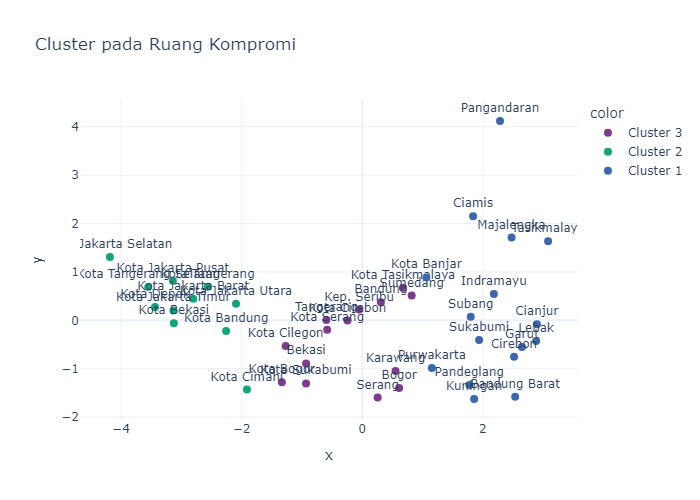
\includegraphics[width=0.9\textwidth]{huggingface/cluster_compromise_biplot.png}
    \caption{Biplot Kompromi Indikator Ekonomi dan Kabupaten/Kota}
    \label{fig:compromise_biplot}
\end{figure}

Interpretasi Sumbu Utama:
\begin{enumerate}
    \item \textbf{Sumbu Horizontal (Dimensi 1):} Menjelaskan ...\% variansi data. Sumbu ini berkorelasi kuat dengan variabel [Sebutkan Variabel dari Loading], sehingga dapat diinterpretasikan sebagai dimensi "Kesejahteraan \& Infrastruktur". Wilayah di sebelah kanan (seperti Jakarta Pusat, Kota Bandung) memiliki skor tinggi pada dimensi ini.
    \item \textbf{Sumbu Vertikal (Dimensi 2):} Menjelaskan ...\% variansi. Sumbu ini merepresentasikan "Ketimpangan/Kemiskinan" [Sesuaikan dengan variabel yang vektornya ke atas].
\end{enumerate}

\subsection{\normalsize Pengujian Pola Spasial (Moran's I)}
Untuk menguji apakah sebaran nilai skor pada Sumbu Kompromi 1 (Kesejahteraan \& Infrastruktur) memiliki pola geografis tertentu, dilakukan uji autokorelasi spasial global (Moran's I).

Hasil perhitungan menunjukkan nilai Moran's I sebesar \textbf{0.7252}, yang jauh melampaui nilai ekspektasi ($E[I] = -0.0250$). Hal ini mengindikasikan adanya pola pengelompokan spasial (\textit{spatial clustering}) yang kuat dan positif. Artinya, kabupaten/kota dengan kinerja ekonomi tinggi cenderung bertetangga dengan wilayah berkinerja tinggi lainnya (misalnya klaster Jabodetabek), begitu pula wilayah dengan kinerja rendah cenderung mengelompok dengan sesamanya. Temuan ini menegaskan bahwa kinerja ekonomi di wilayah studi tidak menyebar secara acak, melainkan dipengaruhi secara signifikan oleh faktor lokasi geografis (\textit{neighborhood effect}).


%-----------------------------------------------------------------------------%
% --- 4.4 ---
\section{\normalsize Uji Stabilitas (Permutation Test)}
%-----------------------------------------------------------------------------%
Untuk memvalidasi apakah struktur kompromi tersebut signifikan secara statistik dan bukan terbentuk secara kebetulan, dilakukan uji permutasi dengan $B=1000$ iterasi.

\begin{figure}[htbp]
    \centering
    % \includegraphics[width=0.7\textwidth]{gambarku/permutation_plot.png}
    % TODO: Screenshot grafik Histogram Permutasi dari Dashboard
    \caption{Distribusi Null Nilai Eigen Pertama dari Uji Permutasi}
    \label{fig:perm_test}
\end{figure}

Hasil pengujian menunjukkan nilai eigen pertama observasi ($\theta_1^{obs}$) berada jauh di luar area distribusi null ($p$-value $< 0.05$). Hal ini membuktikan hipotesis penelitian bahwa terdapat struktur ekonomi multivariat yang stabil dan nyata (\textit{statistically significant}) di wilayah studi selama periode 2020--2024.

%-----------------------------------------------------------------------------%
% --- 4.5 ---
\section{\normalsize Analisis Dinamika Spasio-Temporal (Trajectories)}
%-----------------------------------------------------------------------------%
Bagian ini menganalisis pergeseran posisi (nasib) kabupaten/kota spesifik dari masa krisis menuju pemulihan.

\begin{figure}[htbp]
    \centering
    % \includegraphics[width=1.0\textwidth]{gambarku/trajectories_2d.png}
    % TODO: Screenshot "STATIS Trajectories" dari Dashboard
    \caption{Peta Lintasan Perubahan Ekonomi Kabupaten/Kota (2020--2024)}
    \label{fig:traj_map}
\end{figure}

\subsection{\normalsize Pola Pemulihan Kota Metropolitan (V-Shape)}
Kota-kota berbasis jasa seperti Jakarta Pusat dan Kota Bandung menunjukkan pola lintasan "memantul" (\textit{rebound}). Pada tahun 2020, posisi mereka bergeser ke arah ... [Jelaskan arah pergeseran di grafik], mencerminkan kontraksi ekonomi. Namun, pada 2022--2024, mereka bergerak kembali ke posisi awal atau bahkan lebih tinggi, menandakan pemulihan yang kuat.

\subsection{\normalsize Pola Stagnasi Wilayah Penyangga}
Berbeda dengan kota metropolitan, wilayah penyangga seperti Kabupaten Lebak atau Pandeglang menunjukkan pergerakan trajektori yang relatif pendek (statis). Hal ini mengindikasikan bahwa perubahan makroekonomi maupun pemulihan tidak memberikan dampak perubahan struktural yang signifikan pada kesejahteraan relatif wilayah tersebut.

%-----------------------------------------------------------------------------%
% --- 4.6 ---
\section{\normalsize Analisis Klaster Spasio-Temporal}
%-----------------------------------------------------------------------------%
Untuk mendapatkan wawasan mendalam mengenai pengelompokan tahunan dan perpindahannya, dilakukan analisis clustering pada skor utama PCA (PC1 dan PC2) di setiap tahun.

\subsection{\normalsize Penentuan Jumlah Klaster (\texorpdfstring{$k$}{k})}
Penentuan jumlah klaster optimal dilakukan secara empiris dengan memadukan Metode \textit{Elbow} dan \textit{Agglomerative Hierarchical Clustering} (Dendrogram).

\begin{figure}[htbp]
    \centering
    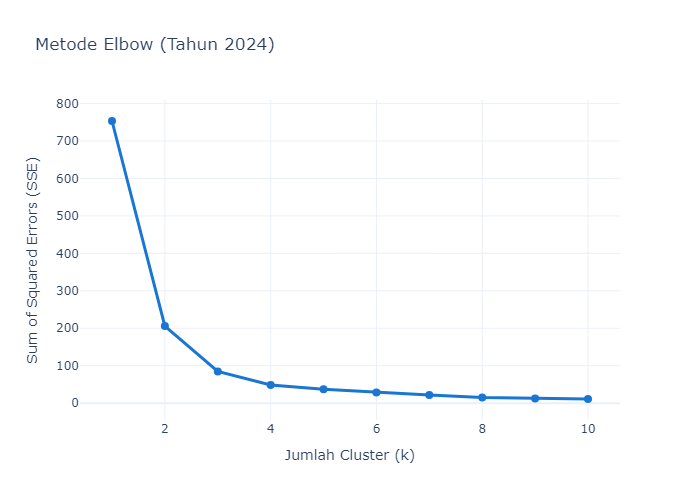
\includegraphics[width=0.45\textwidth]{huggingface/elbow_plot_2024.png}
    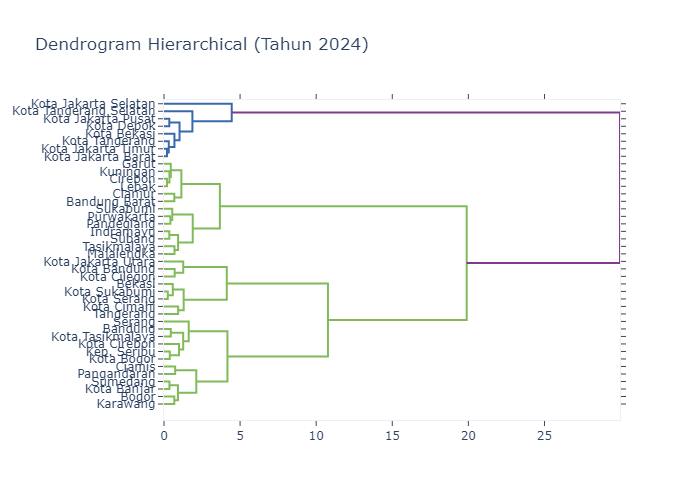
\includegraphics[width=0.45\textwidth]{huggingface/dendrogram_2024.png}
    \caption{Kurva Elbow dan Dendrogram (Tahun 2024)}
    \label{fig:elbow_dendro}
\end{figure}

Berdasarkan titik patahan (\textit{elbow}) pada kurva SSE dan evaluasi tinggi cabang pada dendrogram di Gambar \ref{fig:elbow_dendro}, jumlah klaster $k = \dots$ dipilih sebagai partisi optimal untuk tahun-tahun pengamatan.

\subsection{\normalsize Pola Pengelompokan dan Matriks Transisi}
Hasil pengelompokan membagi wilayah ke dalam $k$ klaster (misalnya: Klaster Kesejahteraan Tinggi, Menengah, dan Rendah). 

\begin{figure}[htbp]
    \centering
    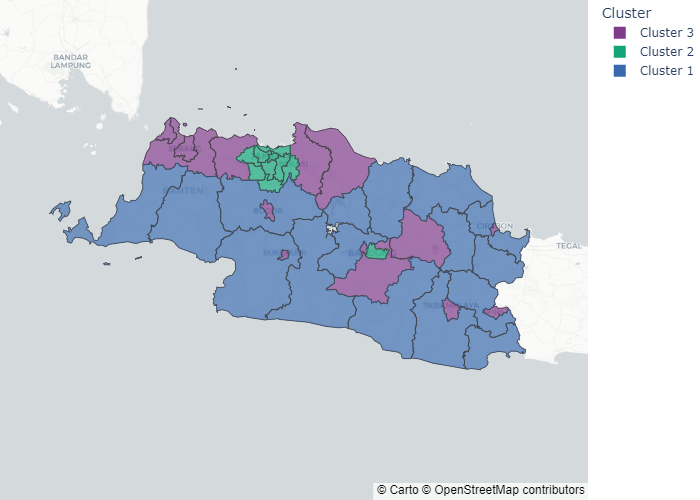
\includegraphics[width=0.9\textwidth]{huggingface/cluster_map_2024.png}
    \caption{Peta Sebaran Klaster Kabupaten/Kota (Tahun 2024)}
    \label{fig:cluster_map}
\end{figure}

Untuk menganalisis dinamika perubahan nasib (migrasi klaster) wilayah antara tahun terburuk pandemi (2020) dengan fase pemulihan, dibentuk suatu matriks perpindahan silang (\textit{transition matrix}).

\begin{table}[H]
\centering
\caption{Matriks Transisi Klaster Tahun 2020 ke 2021} \label{tab:transisi_2020_2021}
\begin{tabular}{|c|p{2cm}|p{2cm}|p{2cm}|}
\hline
\textbf{Tahun 2020 \\ 2021} & \textbf{Cluster 1 (2021)} & \textbf{Cluster 2 (2021)} & \textbf{Cluster 3 (2021)} \\ \hline
\textbf{Cluster 1 (2020)} & 16 & 0 & 2 \\ \hline
\textbf{Cluster 2 (2020)} & 0 & 1 & 11 \\ \hline
\textbf{Cluster 3 (2020)} & 0 & 11 & 0 \\ \hline
\end{tabular}
\end{table}

Berdasarkan tabel matriks transisi di atas, sebagian besar wilayah (\dots kabupaten/kota) masih menetap di klasternya masing-masing (berada di diagonal utama). Namun, terdapat \dots wilayah yang berhasil naik "kelas" (bermigrasi ke klaster yang lebih baik) seiring dengan program pemulihan ekonomi daerah.

\subsection{\normalsize Evaluasi Klaster terhadap Kategori IPM (UNDP)}
Sebagai \textit{baseline} evaluasi, pengelompokan K-Means dibandingkan dengan standar klasifikasi Indeks Pembangunan Manusia (IPM) dari UNDP. Berikut adalah tabel dinamika transisi wilayah berdasarkan kategori IPM.

\begin{table}[H]
\centering
\caption{Matriks Transisi IPM Tahun 2020 ke 2021} \label{tab:ipm_transisi_2020_2021}
\begin{tabular}{|c|p{2cm}|p{2cm}|p{2cm}|p{2cm}|}
\hline
\textbf{Tahun 2020 \\ 2021} & \textbf{Sangat Tinggi (2021)} & \textbf{Tinggi (2021)} & \textbf{Sedang (2021)} & \textbf{Rendah (2021)} \\ \hline
\textbf{Sangat Tinggi (2020)} & 9 & 0 & 0 & 0 \\ \hline
\textbf{Tinggi (2020)} & 0 & 18 & 0 & 0 \\ \hline
\textbf{Sedang (2020)} & 0 & 0 & 14 & 0 \\ \hline
\textbf{Rendah (2020)} & 0 & 0 & 0 & 0 \\ \hline
\end{tabular}
\end{table}

Selanjutnya, untuk memastikan apakah klaster yang dibentuk oleh algoritma \textit{K-Means} selaras dengan kondisi riil di lapangan, dilakukan tabulasi silang (\textit{cross-tabulation}) antara anggota klaster K-Means dengan kategori IPM di tahun akhir pengamatan (2024).

% !TeX root = ../induk.tex
\begin{table}[H]
\centering
\caption{Perbandingan Anggota Cluster dengan Kategori IPM (2024)} \label{tab:ipm_cross_2024}
\begin{tabular}{|c|p{2cm}|p{2cm}|p{2cm}|p{2cm}|}
\hline
\textbf{Cluster K-Means} & \textbf{Sangat Tinggi} & \textbf{Tinggi} & \textbf{Sedang} & \textbf{Rendah} \\ \hline
\textbf{Cluster 1} & 0 & 7 & 9 & 0 \\ \hline
\textbf{Cluster 2} & 10 & 0 & 0 & 0 \\ \hline
\textbf{Cluster 3} & 1 & 13 & 1 & 0 \\ \hline
\end{tabular}
\end{table}

Dari tabulasi silang di atas, terlihat bahwa wilayah pada Klaster \dots didominasi oleh daerah dengan kategori IPM "Sangat Tinggi" dan "Tinggi", yang secara empiris memvalidasi bahwa penamaan label klaster tersebut sebagai kelompok "Maju/Sejahtera" sudah sangat tepat.

% !TeX root = induk.tex
\chapter{\normalsize KESIMPULAN DAN SARAN}
\raggedbottom

Bab ini menyimpulkan hasil temuan utama dari analisis STATIS dan Dynamic Biplot mengenai dinamika pembangunan ekonomi regional di Provinsi Banten, DKI Jakarta, dan Jawa Barat, serta memberikan saran rekomendasi kebijakan maupun pengembangan penelitian selanjutnya.

%-----------------------------------------------------------------------------%
% --- 5.1 ---
\section{\normalsize Kesimpulan}
%-----------------------------------------------------------------------------%
Berdasarkan hasil analisis dan pembahasan yang telah dilakukan, dapat ditarik beberapa kesimpulan sebagai berikut:

\begin{enumerate}
    \item \textbf{Karakteristik Struktur Kompromi (Menjawab Tujuan 1):}
    Melalui sintesis matriks kompromi STATIS (Skenario 1 $\mathbf{W}_c$ dan Skenario 2 $\mathbf{S}_c$), diperoleh representasi rata-rata spasio-temporal yang stabil selama periode 2020--2024. Dua dimensi utama berhasil diidentifikasi: Dimensi~1 merepresentasikan ``Taraf Ekonomi dan Kualitas Sumber Daya Manusia'' (didominasi oleh kontribusi positif dari indikator PDRB, IPM, RLS, dan IPG) serta menjelaskan bagian terbesar variansi total (\AppDimOnePct{}\%). Dimensi~2 merepresentasikan ``Kesehatan dan Ketahanan Sosial'' (didominasi oleh Angka Harapan Hidup L/P dan PKKP). Vektor bobot interstruktur ($\boldsymbol{\alpha}_W$ dan $\boldsymbol{\alpha}_S$) terdistribusi secara seimbang di antara kelima tahun pengamatan, yang membuktikan representativitas yang adil tanpa distorsi tahun ekstrem.

    \item \textbf{Signifikansi Stabilitas Temporal dan Vektor Struktur (Menjawab Tujuan 2):}
    Analisis interstruktur STATIS menghasilkan koefisien RV yang sangat tinggi (seluruhnya di atas $\AppRVMin{}$), membuktikan bahwa hierarki kemiripan antar-wilayah bersifat persisten lintas waktu. Uji permutasi Monte Carlo ($B = 1000$) membuktikan bahwa struktur kompromi tersebut \textbf{signifikan secara statistik} ($p\text{-value} = \AppPValuePerm{} < 0{,}05$) dan bukan merupakan hasil fluktuasi acak. Kompresi interstruktur ke dalam vektor struktur $\tilde{\boldsymbol{\beta}} = \lambda_1 \boldsymbol{\alpha}_1$ secara longitudinal merekam dampak krisis pandemi (2020--2021) dan pemulihan (2022--2024) yang nyata, sementara analisis transversal membuktikan adanya heterogenitas respons temporal yang unik antar-provinsi.

    \item \textbf{Pola Lintasan Trajektori Spasio-Temporal (Menjawab Tujuan 3):}
    Visualisasi \textit{Dynamic Biplot} berhasil menggambarkan lintasan (\textit{trajectory}) pergerakan 41 kabupaten/kota secara dinamis dari masa krisis (2020) hingga masa pemulihan (2024). Tiga pola pergerakan diidentifikasi: (1) pola pemulihan berbentuk huruf V (\textit{V-shape rebound}) pada kota-kota metropolitan berbasis jasa (seperti DKI Jakarta, Kota Bandung, Kota Tangerang Selatan), (2) pola progresif bertahap (\textit{monotone improvement}) pada wilayah penyangga, dan (3) pola stagnasi (\textit{inertia}) pada kabupaten pedalaman bagian selatan (seperti Lebak, Pandeglang, Garut) yang respons pemulihannya lambat.

    \item \textbf{Pengelompokan Spasial dan Dinamika Transisi (Menjawab Tujuan 4):}
    Penerapan algoritma K-Means ($k=3$) pada skor kompromi berhasil mengklasifikasikan wilayah secara objektif menjadi tiga kelompok: Klaster~1 (Tertinggal/Banten Selatan dan pedalaman), Klaster~2 (Berkembang/Wilayah penyangga), dan Klaster~3 (Maju/Metropolitan). Matriks transisi temporal lintas tahun mengonfirmasi dominasi diagonal utama yang sangat tinggi (stabilitas pengelompokan yang kokoh), namun tetap menangkap adanya mobilitas naik (\textit{upward migration}) yang selektif pada wilayah tertentu (seperti Kabupaten Kepulauan Seribu yang bermigrasi dari Klaster 1 ke Klaster 2 pada tahun 2023).

    \item \textbf{Pengembangan Dashboard Eksplorasi Interaktif (Menjawab Tujuan 5):}
    Aplikasi berbasis web dikembangkan menggunakan \textit{framework} Dash dan Plotly sebagai instrumen eksplorasi visual interaktif yang andal. Fitur-fitur seperti pemetaan spasial dinamis, visualisasi trajektori, seleksi tahun, dan rotasi sumbu \textit{baseline} berhasil memfasilitasi pemantauan indikator pembangunan secara interaktif oleh peneliti dan pemangku kebijakan. Keandalan model terkonfirmasi melalui validasi eksternal (tabulasi silang) yang menunjukkan kesesuaian yang sangat tinggi antara klaster STATIS dengan klasifikasi normatif kategori IPM UNDP.
\end{enumerate}

%-----------------------------------------------------------------------------%
% --- 5.2 ---
\section{\normalsize Saran}
%-----------------------------------------------------------------------------%
Berdasarkan kesimpulan di atas, diajukan beberapa saran sebagai berikut:

\begin{enumerate}
    \item \textbf{Implikasi Kebijakan \textit{Targeted} Regional:}
    Mengingat struktur ketimpangan yang persisten dan terpola secara spasial, kebijakan pemerataan pembangunan tidak cukup hanya mengandalkan pertumbuhan ekonomi nasional. Diperlukan intervensi struktural yang \textit{targeted} pada wilayah Klaster~1 (Tertinggal), khususnya Kabupaten Lebak, Pandeglang, dan Garut, dengan fokus pada peningkatan kapabilitas dasar (RLS, AHH) serta pengurangan kemiskinan melalui strategi \textit{regional spillover} dari pusat pertumbuhan DKI Jakarta.
    
    \item \textbf{Pengembangan Penelitian Lanjutan:}
    Penelitian ini dibatasi pada indikator makroekonomi tahunan dari 3 provinsi. Penelitian selanjutnya disarankan untuk menggunakan data dengan resolusi waktu yang lebih tinggi (triwulanan) apabila tersedia, memperluas cakupan wilayah ke seluruh Pulau Jawa atau Indonesia dengan mengintegrasikan metode \textit{Dual STATIS} untuk analisis korelasi indikator, serta menambahkan indikator sosial-infrastruktur guna memperkaya dimensi analisis.

    \item \textbf{Pengembangan Model Prediktif Spasio-Temporal (\textit{Forecasting}):}
    Karena penelitian ini terbatas pada analisis deskriptif-eksploratif data historis, penelitian selanjutnya sangat disarankan untuk mengintegrasikan model prediktif (peramalan) guna memproyeksikan skor wilayah ($F_k$) dan loading indikator ($G_k$) ke tahun berikutnya ($k = K+1$). Hal ini dapat diwujudkan dengan menerapkan pemodelan deret waktu (seperti ARIMA, Vector Autoregression (VAR), atau model \textit{Grey Systems} GM(1,1) yang sangat handal untuk deret data pendek $K=5$) langsung pada barisan koordinat kompromi ($\mathbf{f}_{i,k}$ dan $\mathbf{g}_{j,k}$) dan lintasan komponen vektor struktur ($\tilde{\beta}_k$). Dengan memproyeksikan lintasan koordinat ini, pemangku kebijakan dapat mengantisipasi pergeseran status kesejahteraan wilayah dan dinamika hubungan antar-indikator secara prospektif.

    \item \textbf{Pengembangan Platform \textit{Dashboard} Interaktif:}
    Dashboard berbasis web (Dash/Plotly) yang dikembangkan dalam penelitian ini dapat dikembangkan lebih lanjut dengan menambahkan fitur pembaruan data secara otomatis dari API BPS Open Data, sehingga pemantauan dinamika pembangunan regional dapat dilakukan secara \textit{near real-time} oleh pemangku kepentingan kebijakan.
\end{enumerate}



% Daftar Pustaka
%Buat daftar pustaka
\bibliographystyle{apalike-ejor}
\bibliography{pustaka} % Tambahkan pustaka yang digunakan mahasiswa dalam file pustaka.bib. Perhatikan format penulisan pustakanya!

% Lampiran (jika ada)

\begin{appendix}
	%
% @author  Andreas Febrian
% @version 1.00 
% 
% Hanya sebuah pembatas bertuliskan LAMPIRAN ditengah halaman. 
% 

\begin{titlepage}
	\centering 
	\vspace*{6cm}
	\noindent \Huge{LAMPIRAN}
	\addChapter{LAMPIRAN}
\end{titlepage}
	\addChapter{Lampiran 1}
\chapter*{\normalsize Lampiran 1}

Perhatikan penurunan model berikut.
\end{appendix}
\end{document} 
